\documentclass{article}
\usepackage[margin=.5in]{geometry}
\usepackage{graphicx, dblfloatfix}
\usepackage{amsmath, amssymb, amsfonts, mathrsfs, mathtools, physics}
\usepackage[english]{babel}
\usepackage[autostyle, english = american]{csquotes}
\usepackage[normalem]{ulem}
\usepackage[title,titletoc,toc]{appendix}
\usepackage{pgfplotstable}
\usepackage{array, booktabs, colortbl}
\MakeOuterQuote{"}

\pgfplotsset{compat=1.12}


\newcommand{\redchi}{$\tilde{\chi}^2\,$}
\DeclareMathOperator{\cov}{cov}
\DeclarePairedDelimiter{\parens}{\lparen}{\rparen}

\title{Neutron Studies}
\author{Aman LaChapelle}

\begin{document}
\raggedright
\maketitle

\begin{abstract}
  Here we show a method by which we can measure an effective radius for the neutron, as well as observe the reaction that creates a deuteron.  We demonstrate techniques which can be used in order to perform these measurements using fast neutrons emitted from a PuBe source.
\end{abstract}

\tableofcontents
\newpage

\section{Introduction}
  In this experiment we demonstrate means by which we are able to observe the reaction that creates a deuteron, as well as measuring the size of the neutron.  We collect data for multiple thicknesses of each absorber in order to determine the scattering cross-section of the fast neutrons as they pass through the absorbers.  Based on the intensity of neutrons that hit the plastic scintillator detector, we are able to determine how many were absorbed or back-scattered.  From this intensity, we are able to calculate the size of the nucleus since neutrons will scatter only if they pass within about one wavelength (the neutron's de Broglie wavelength) of the nucleus.  Thus, based on the proportion of neutrons that pass through the absorber we will be able to determine an approximate density (and thus size) for the nuclei of that absorber.

\section{Theory}
  \subsection{Deuteron Production}
  There is a stable bound state of a proton and a neutron called a deuteron.  In general, if the neutron has energy comparable to the proton, it will be possible to have the neutron hit the proton and create this bound state.  It differs from deuterium in that it does not necessarily have the bound electron that a hydrogen atom typically does.  The important concept to note is that the deuteron is a bound state of a neutron and of a proton.  This state has lower energy than the sum of the incoming energy of the neutron and proton, and so the reaction that creates a deuteron is characterized by a capture photon on the order of 2 MeV.  Since the neutrons and protons that have low enough energy to fall into a bound state like this one are generally barely moving if at all, we take their energy to be roughly equal to their rest mass for the purposes of a rough calculation.  Use the following reaction:
  \begin{equation*}
    n + p \rightarrow d + \gamma
  \end{equation*}
  We determine that given the rest energy of the neutron, proton, and deuteron, the capture photon should have an energy of around 2.1 MeV.

  \hspace{.25cm}

  Experimentally, this reaction is not particularly simple to measure.  However, we take a hydrogen-rich substance - paraffin - and place it in the path of the fast neutrons.  We then place that in front of our detector which we expect to measure the capture photons.  However, there is a lot of ambient energy, which translates into a lot of ambient photons.  This translates into, experimentally, shielding the detector with lead bricks in order to attenuate photons coming from the paraffin surrounding the PuBe core, or even ambient lighting, for example.  Thus we take a series of spectra to determine background rates, and we will perform a check to make sure that the deuteron production is actually occurring with the hydrogen atoms in the paraffin and not (for example) the creation and decay of Carbon-13.

  \subsection{Neutron Cross-Section/Nucleus Size}
  Neutrons typically interact with low-Z materials - that is, they interact with materials that have a comparable atomic size/mass to the neutron.  Carbon is heavier, but only by an order of magnitude.  What this means is that carbon is a good attenuator of these fast neutrons.  What it will not do, however, is to give off the capture photons that we got used to in the first part of the experiment, as will happen when the neutron interacts with a hydrogen nucleus to create a deuteron.  Thus, in order to measure the attenuation rate of neutrons due to different materials (in order to determine a cross-section), we will have to look at continuous data.  We fit our PMT with a plastic scintillator.  The incoming fast neutrons will scatter the hydrogen atoms in the plastic and cause light emission.  These light emissions are seen by the PMT and translated into voltage pulses that allow us to measure the energy deposited by the scattered protons (and thus, roughly, the incoming neutrons).

  \hspace{.25cm}

  The detector is sensitive to incoming photons as well, however, its response is different, which allows us to find an effective region of interest for which the response is due to protons and not to incident photons.  In Figure~\ref{response} we can see that the response for a 7 MeV proton is roughly 3 times the response of a 1.275 MeV photon.  Since we have access to Na-22 sources which emit 1.275 MeV photons as one of their full energy peaks, we are able to perform a sort of calibration on the axis and roughly determine a region of interest by looking for the Compton edges on the Na-22 spectrum and using a ROI that begins at roughly 3 times the 1.275 MeV Compton edge and goes to the end of the detector range, as we can see in Figure~\ref{roi}.

  \hspace{.25cm}

  We can perform a rough calculation in determining the region of interest if we consider the Compton edge.  Given the Compton formula,

  \begin{equation*}
    E' = \frac{E}{1+\frac{E}{mc^2}\parens*{1-\cos{\theta}}}
  \end{equation*}

  and given that the scattering angle is going to be roughly $\pi$, we can therefore calculate an approximate energy for the scattered photon $E'$ given input energies.  If we calculate $E'$ for a proton of energy that is approximately 7 MeV and for an electron of 1 MeV, and take the quotient, we return a value of 3, as we can read from Figure~\ref{response}. Thus we can be certain we will set our ROI to begin at the channel that is 3 times the Na-22 1275 keV Compton edge.

  \hspace{.25cm}

  In actually collecting data, we shield the detector with approximately 4 inches of lead in order to attenuate any photons that are coming either from the paraffin shield around the PuBe source or any other sources in the room.  We are interested in the count rate of neutrons as they pass through various absorbers, and as such we are \textbf{not} interested in the counts that we gain from other, ambient sources.  In this spirit, we measure the ambient background by blocking the detector from the source with approx. 28 inches of Pb.  We can then integrate the region of interest for each absorber element and thickness in order to determine a cross section for the absorbers.  From this, we will be able to calculate an effective radius for the neutron.

  \hspace{.25cm}

  The Ramsauer model suggests that nuclei present a cross section that is equal to twice their effective area.  That is,
  \begin{equation*}
    \sigma = 2\pi\parens*{R + \lambda}^2
  \end{equation*}
  where $R$ is the radius, and $\lambda$ is the deBroglie wavelength of the neutron.  According to this model, scattering only occurs if the neutron passes within about 1 wavelength of the nucleus.  This means that the radius of the nucleus roughly obeys the rule
  \begin{equation*}
    R = r_0A^{1/3}
  \end{equation*}
  which implies that
  \begin{equation*}
    \sqrt{\frac{\sigma}{2\pi}} = r_0 A^{1/3} + \lambda
  \end{equation*}
  where $r_0$ is the radius of the neutron and $A$ is the average atomic mass.  We should thus be able to, given accurate cross sections, determine the radius of the neutron by plotting $\sqrt{\frac{\sigma}{2\pi}}$ versus $A^{1/3}$, fitting a line and extracting the slope and intercept of that line.  Those two parameters should return the radius and the deBroglie wavelength of a neutron, respectively.

\section{Experimental Procedure, Data and Uncertainty Analysis}
  It should be mentioned that unless otherwise mentioned, all the plot uncertainties are from counting, so we estimate them as $\sqrt{n}$.
  \subsection{Neutron Mass}
  The first step for this portion of the experiment was to calibrate the channel axis on the PHA.  The software generally collects data as counts versus channel, but each channel corresponds to an energy - the question is what energy does it correspond to.  In order to calibrate this axis, we take several sources that emit photons at known energies with high consistency and use these to calibrate the axis.  As we can see in Figure~\ref{cal_peaks}, this produces an excellent calibration of the channel axis as long as we know the peak locations and what energies they correspond to with high precision.  Given such a high precision measurement, we are able to calibrate the axis quite well.  In order to make sure that our numbers are good, we took the first fit and randomly chose guess parameters from a normal distribution centered at the best-fit parameters.  In this way we were able to make sure that the fit shown corresponds to the best fit possible.

  \hspace{.25cm}

  Now that we actually have the peak locations, and we know what the energies correspond to, we are able to fit a line through these points in order to determine the calibration from channel to energy, as we can see in Figure~\ref{calibration}.  The linewidth and point size were chosen to represent the relative size of the uncertainty in the slope and points, respectively.  As we can see, both are quite small.  Thus the uncertainties that come up in our calibration will be negligible going forward - we can trust that our calibration is true.

  \hspace{.25cm}

  In order to take measurements, we perform a series of tests in order to determine things like background counts, how well the lead attenuates photons from the source shielding (Figure~\ref{apparatus}), and other factors.  The first measurement we make is with the open detector, no lead shielding, with the port open and then with the port closed.  We see that the count rate of photons is quite similar - the photon source is the shielding of the PuBe source - as we can see in Figure~\ref{nolead}.  If we now shield the detector with lead in order to determine background counts, we see spectra as shown in Figure~\ref{lead}, both of which are very close to zero.  This effectively gives us a background that we can use to compare further measurements against.  Visually, we will be able to see if the peaks are better-defined and/or larger than these then we actually have a peak and thus a valid countrate.

  \hspace{.25cm}

  We compare measurements from two different experimental setups (Figure~\ref{apparatus}).  In the space between the lead and the NaI detector, we put 6 inches of carbon or paraffin.  If we put in paraffin, we observe a peak that reappears at the capture photon energy, and we expect this peak occurs due to the hydrogen in the paraffin, not the carbon.  In order to test this, we will make a measurement of the countrate under the region where we expect to see the capture photon with paraffin in front of the detector.  We will then compare it with blocks of carbon in order to ensure that the reaction is in fact the capture reaction caused by the hydrogen nuclei and not a scattering event off the carbon.  Thus we expect the peak to disappear in the case where we have the carbon in front of the detector.

  \hspace{.25cm}

  Looking at Figure~\ref{paraffin}, we note that the countrate is quite small, but is non-zero.  Furthermore, the peak is easily identifiable.  If we now take a look at Figure~\ref{carbon}, we see that the peak is hardly identifiable at all.  Qualitatively, we can see that there is obviously no peak in the carbon case.  Quantitatively, we can cite the fact that the fitted countrate for the paraffin case is $0.29 \pm 0.01$ and the fitted countrate for the carbon case is $0.07 \pm 0.01$, and these two values are statistically different.  The carbon value is $22\sigma$ away from the paraffin value and it is thus statistically impossible for these two measurements to have 'true' values that are the same.  These two countrates indicate that there is a phenomenon that occurs in the paraffin that does not occur in the carbon that causes an increase in countrate.

  \hspace{.25cm}

  Since we know that there is in fact a capture photon being emitted in the paraffin, we can find the center of that peak and use the energy of the capture photon to determine the mass of the neutron.  The center of the peak (and thus the value for the energy of the capture photon) is $2179 \pm 6\, keV$.  We can take this and plug it into an expresison for the conservation of energy,
  \begin{gather*}
    E_p + E_n = E_d + E_\gamma \\
    m_p + m_n = m_d + \frac{E_\gamma}{c^2} \\
    m_n = m_d + \frac{E_\gamma}{c^2} - m_p \\
    m_n = 1.00862 \pm 0.00002 \, amu
  \end{gather*}
  which is actually quite a good approximation of the literature value of the mass which is 1.00866 amu.  Our value is off by approximately $2\sigma$, which means that approximately 97\% of accurate results will be closer to the literature value, but for an experiment set up with blocks of wax, this is an excellent agreement.  We also quite likely underestimated our uncertainty, however these were the values that the fit returned which is an accurate representation of our experimental results.  At most we would have been within $1\sigma$, but that would be manipulating data and uncertainties because we know what the answer \textit{should be} as opposed to what we \textit{measured}.  This might suggest that there is an external source of uncertainty such as the ambient light or even that we had extra paraffin that attenuated capture photons or some other mechanism entirely.

  \subsection{Neutron Radius}
  Moving on now to measuring the radius of the neutron, we again must calibrate the channel axis, but we only have one feature that we can use to calibrate said axis.  Thus we perform a so-called 1-point calibration.  As described in section 2.2 and in Figure~\ref{roi}, we pick out the Na-22 1275 keV compton edge and choose an ROI that corresponds to the approimate response of the detector to a scattered proton as opposed to the scattered electron from the Na-22 source.  We thus choose the region of interest to be 3 times the value chosen for the Na-22 compton edge.  In order to determine the countrates, we integrate over the region of interest and divide by the livetime.  Uncertainty will come from the the points themselves - each individual point has uncertainty of $\sqrt{n}$ - and the livetime which is less than 0.01\% and is thus negligible.  The countrates' uncertainty comes from taking simulated data drawn from a normal distribution about the real data points with standard distribution equal to the uncertainty on each point.  We then integrate over this simulated data and return the set of values.  Then we repeat the simulation 1500 times.  The average of this set is what we report as our best value, with the standard deviation of the set of simulated values as the uncertainty on the best value.

  \hspace{.25cm}

  We then make measurements of counts versus absorber material and thickness.  If we examine Figure~\ref{rates:rates}, we can see that all the countrates are above the baseline to within uncertainties with the exception of one point on Figure~\ref{rates:rates}.d.  This means that, in general, we don't have to worry about the baseline affecting our measurements.  The uncertainty on the cross sections comes from the sources above - the uncertainty on our best value for the numerical integral over the region of interest.  If we gather the cross sections here,

  \begin{center}
    \begin{tabular}{|c|c|c|c|}
      \hline
      Aluminum & Carbon & Copper & Lead \\ \hline
      $(4.50\pm.45)e-24 \, cm^2$ & $(2.01\pm.33)e-24 \, cm^2$ & $(6.48\pm.14)e-24 \, cm^2$ & $(8.56\pm.36)e-24 \, cm^2$ \\ \hline
    \end{tabular}
  \end{center}
  we see the inkling of a pattern.  Futhermore, we can visually check that the cross-sections decay exponentially as we expect, thus we can continue our previous line of reasoning.  If we recall section 2.2, where we established that this relation
  \begin{equation*}
    \sqrt{\frac{\sigma}{2\pi}} = r_0 A^{1/3} + \lambda
  \end{equation*}
  holds, we realize that if we plot these cross sections versus the average atomic masses we have a method for actually determining the radius of the neutron.

  \hspace{.25cm}

  Having actually done this, plotting $\sqrt{\sigma/2\pi}$ vs $A^{1/3}$, we see that we have a line.  In reference to Figure~\ref{radius}, we see that we can actually extract values for the neutron radius and its deBroglie wavelength.  In actually fitting this line, we will notice that the uncertainties are extremely large.  Furthermore, the \redchi value is too good for the fit.  Thus, the only way to properly find the best-fit line with the information we have is to simulate data and perform thousands of fits.  We thus take a random sampling drawn from a normal distribution about each point with standard deviation equal to the uncertainty in the cross-section.  We then fit the simulated points to a line and perform this action 5000 times.  The average of each fit parameter is reported as the best-fit for that paremeter, and the standard deviation is reported as the uncertainty in that parameter.  We thus extract the following values for the neutron radius and deBroglie wavelength.

  \begin{center}
    \begin{tabular}{|c|c|} \hline
      $r_0\,(fm)$ & $\lambda\,(fm)$ \\ \hline
      $1.5 \pm 0.9$ & $3 \pm 3$ \\ \hline
    \end{tabular}
  \end{center}

  If we take the energy of the incoming neutron to be 7 MeV, we can then find the deBroglie wavelength to be 1.7205 fm.  According to \cite{rad_n}, the radius of the neutron has a radius of between 0.3 fm and 2 fm.  Shockingly, both of our values are within uncertainties of these values.  Our range for the deBroglie wavelength is so large that the value that we calculated is within $0.5\sigma$, in fact.  Our value for the radius is within uncertainties (a separation of $0.56\sigma$) of the 2 fm number - which makes sense because the 2 fm is quoted as an effective radius for the neutron, negative charge to cancel the positive core.

\section{Conclusion}
  From the fact that our data agrees with the model to a confidence level of greater than 67\%, it is fair to say that the model for the neutron's radius and wavelength agrees to the data shockingly well for the number of simplifications that were made to the theory.

  \hspace{.25cm}

  Our thanks to the staff of the Advanced Undergraduate Physics Laboratory, especially Prateek Bajaj for answering our frantic questions about the data collection and reminding us to keep the fingers crossed on our left hands at all times while doing physics.

\begin{thebibliography}{2}
  \bibitem{rad_n}
    Basdevant, J.-L.; Rich, J. and Spiro, M. \emph{Fundamentals in Nuclear Physics}. Heidelberg: Springer, ISBN 0-387-01672-4, 2005.
  \bibitem{lab manual}
  	University of Chicago Department of Physics. "Neutron Studies"  https://wiki.uchicago.edu/display/P211manuals/Neutron+Studies. (Accessed Feb. 15-23, 2016)
\end{thebibliography}

\section{Figures}
  \begin{figure}[!htb]
    \centering
    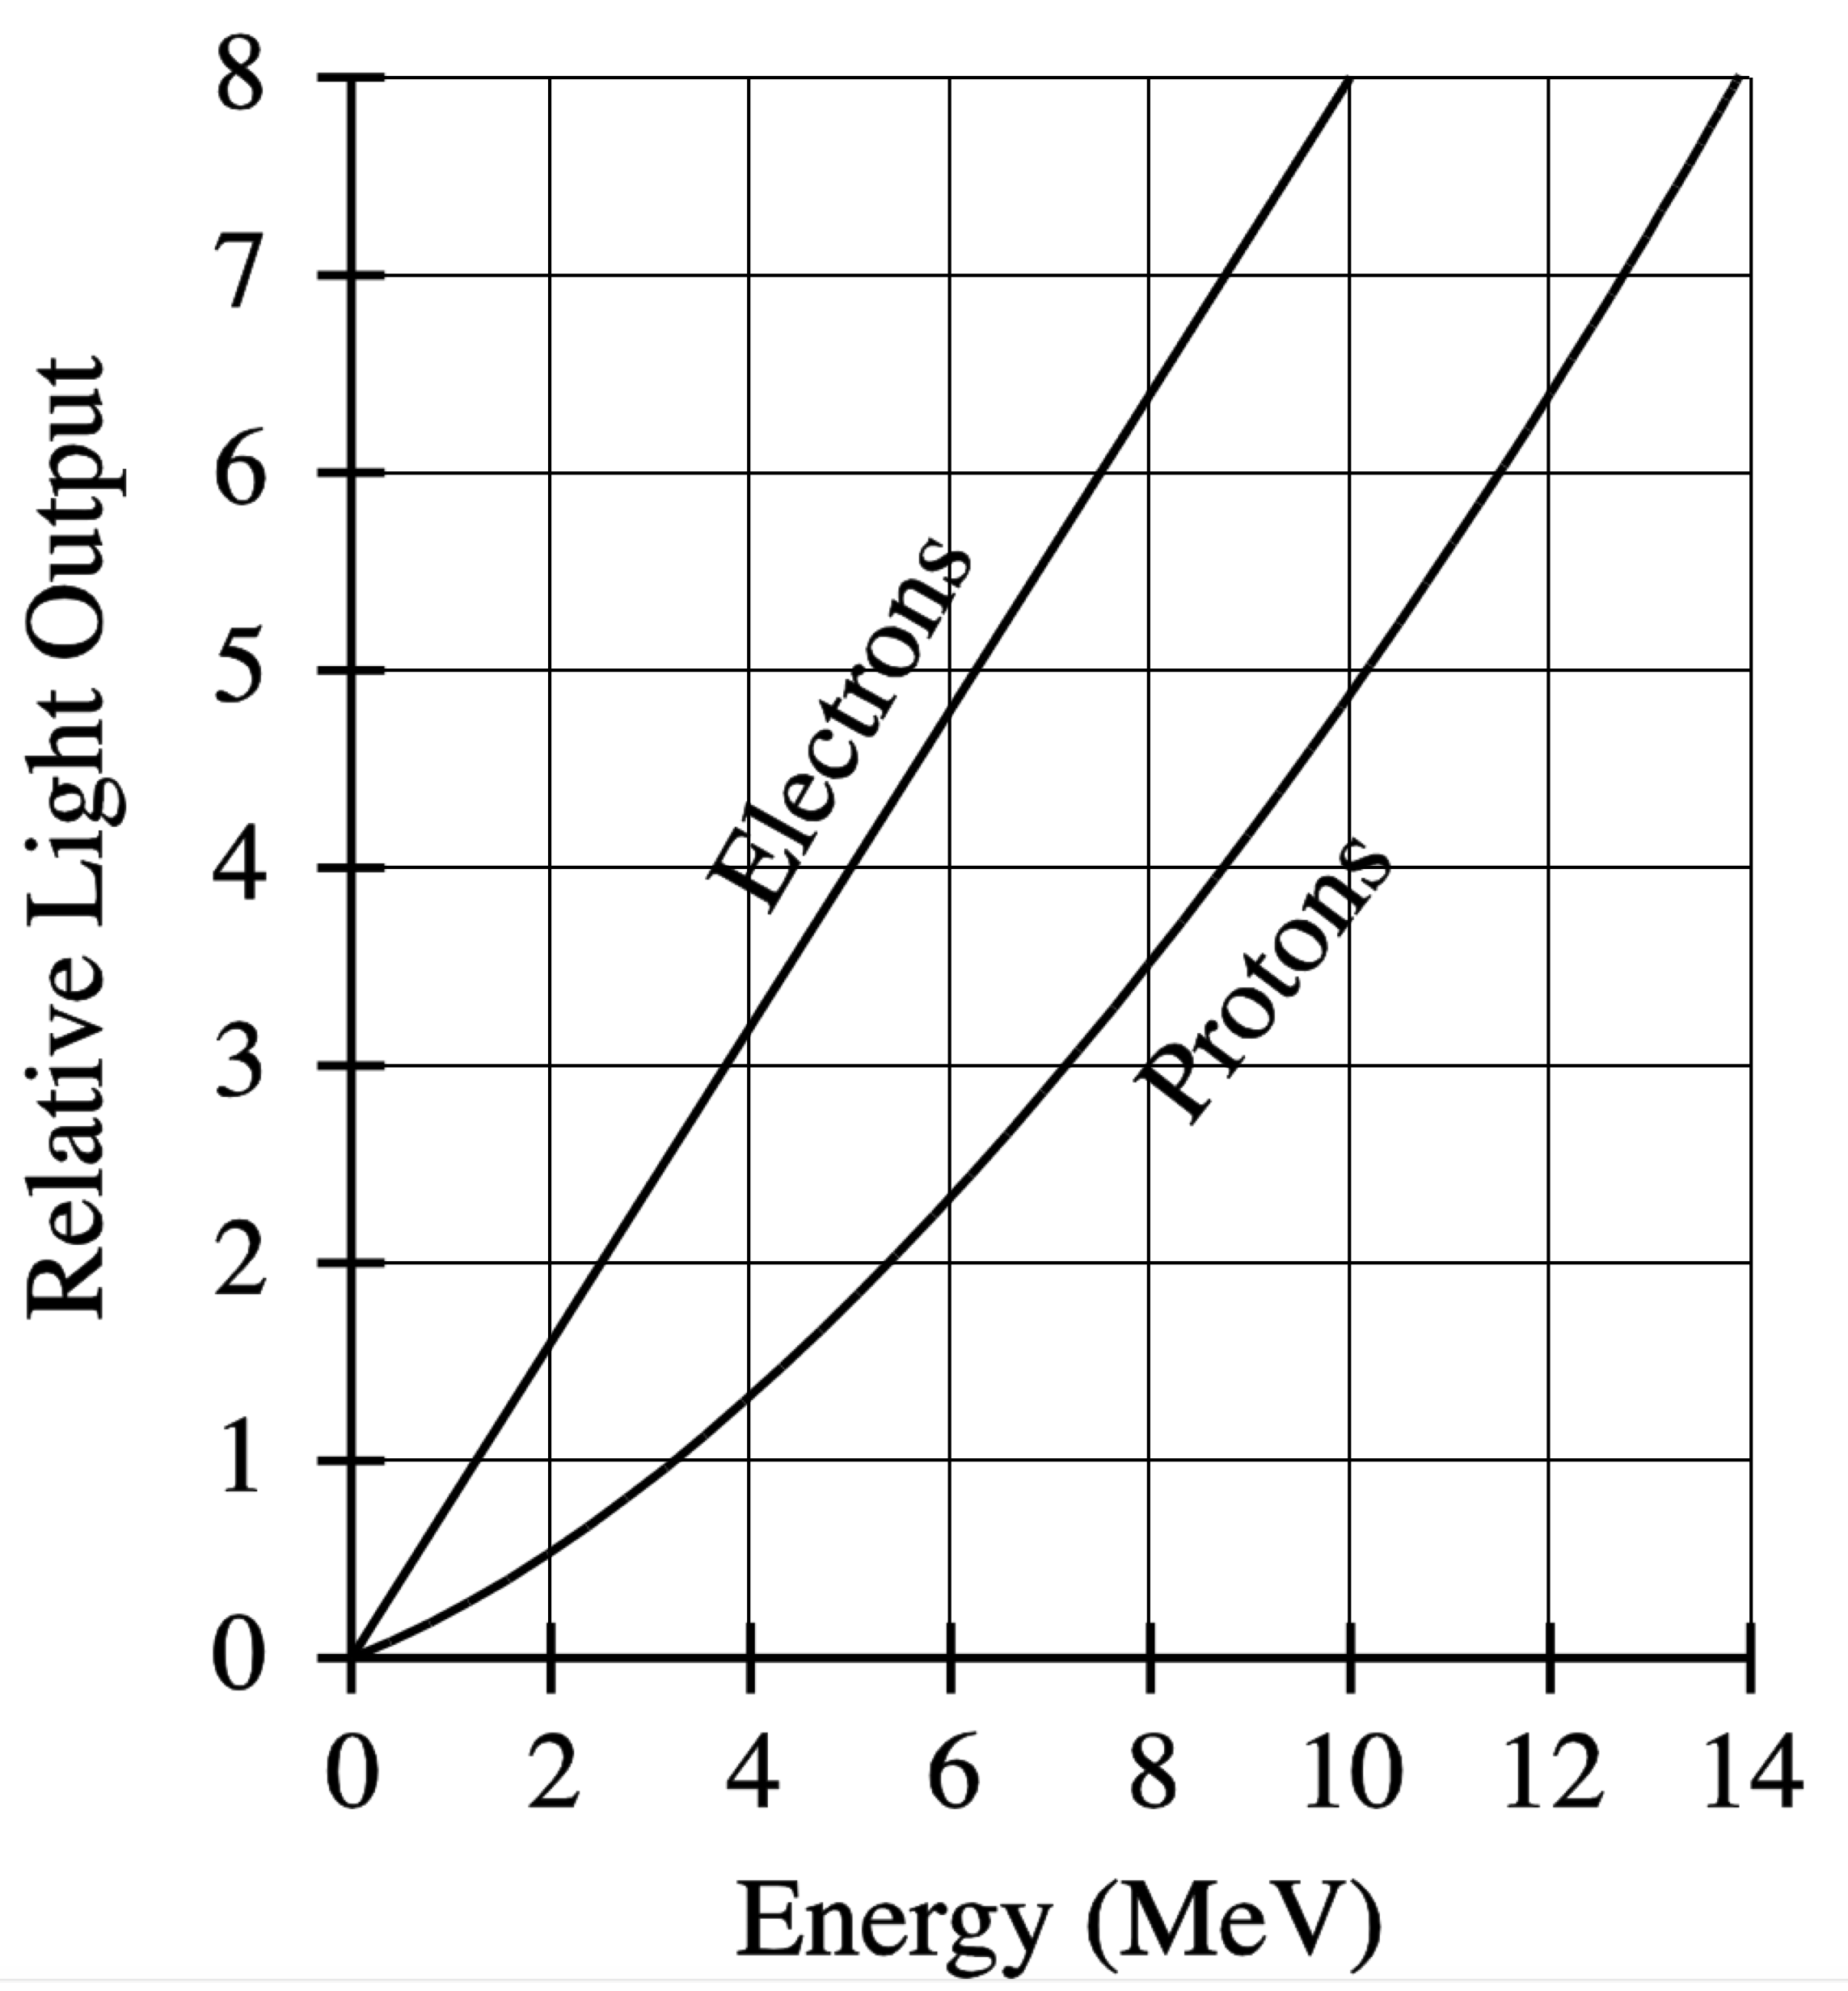
\includegraphics[scale=.5]{relative_response.png}
    \caption{Relative light output resulting from incident photons - which scatter electrons, and from incident neutrons which scatter protons.}
    \label{response}
  \end{figure}

  \hspace{.25cm}

  \begin{figure}[!htb]
    \centering
    \begin{tabular}{c c}
      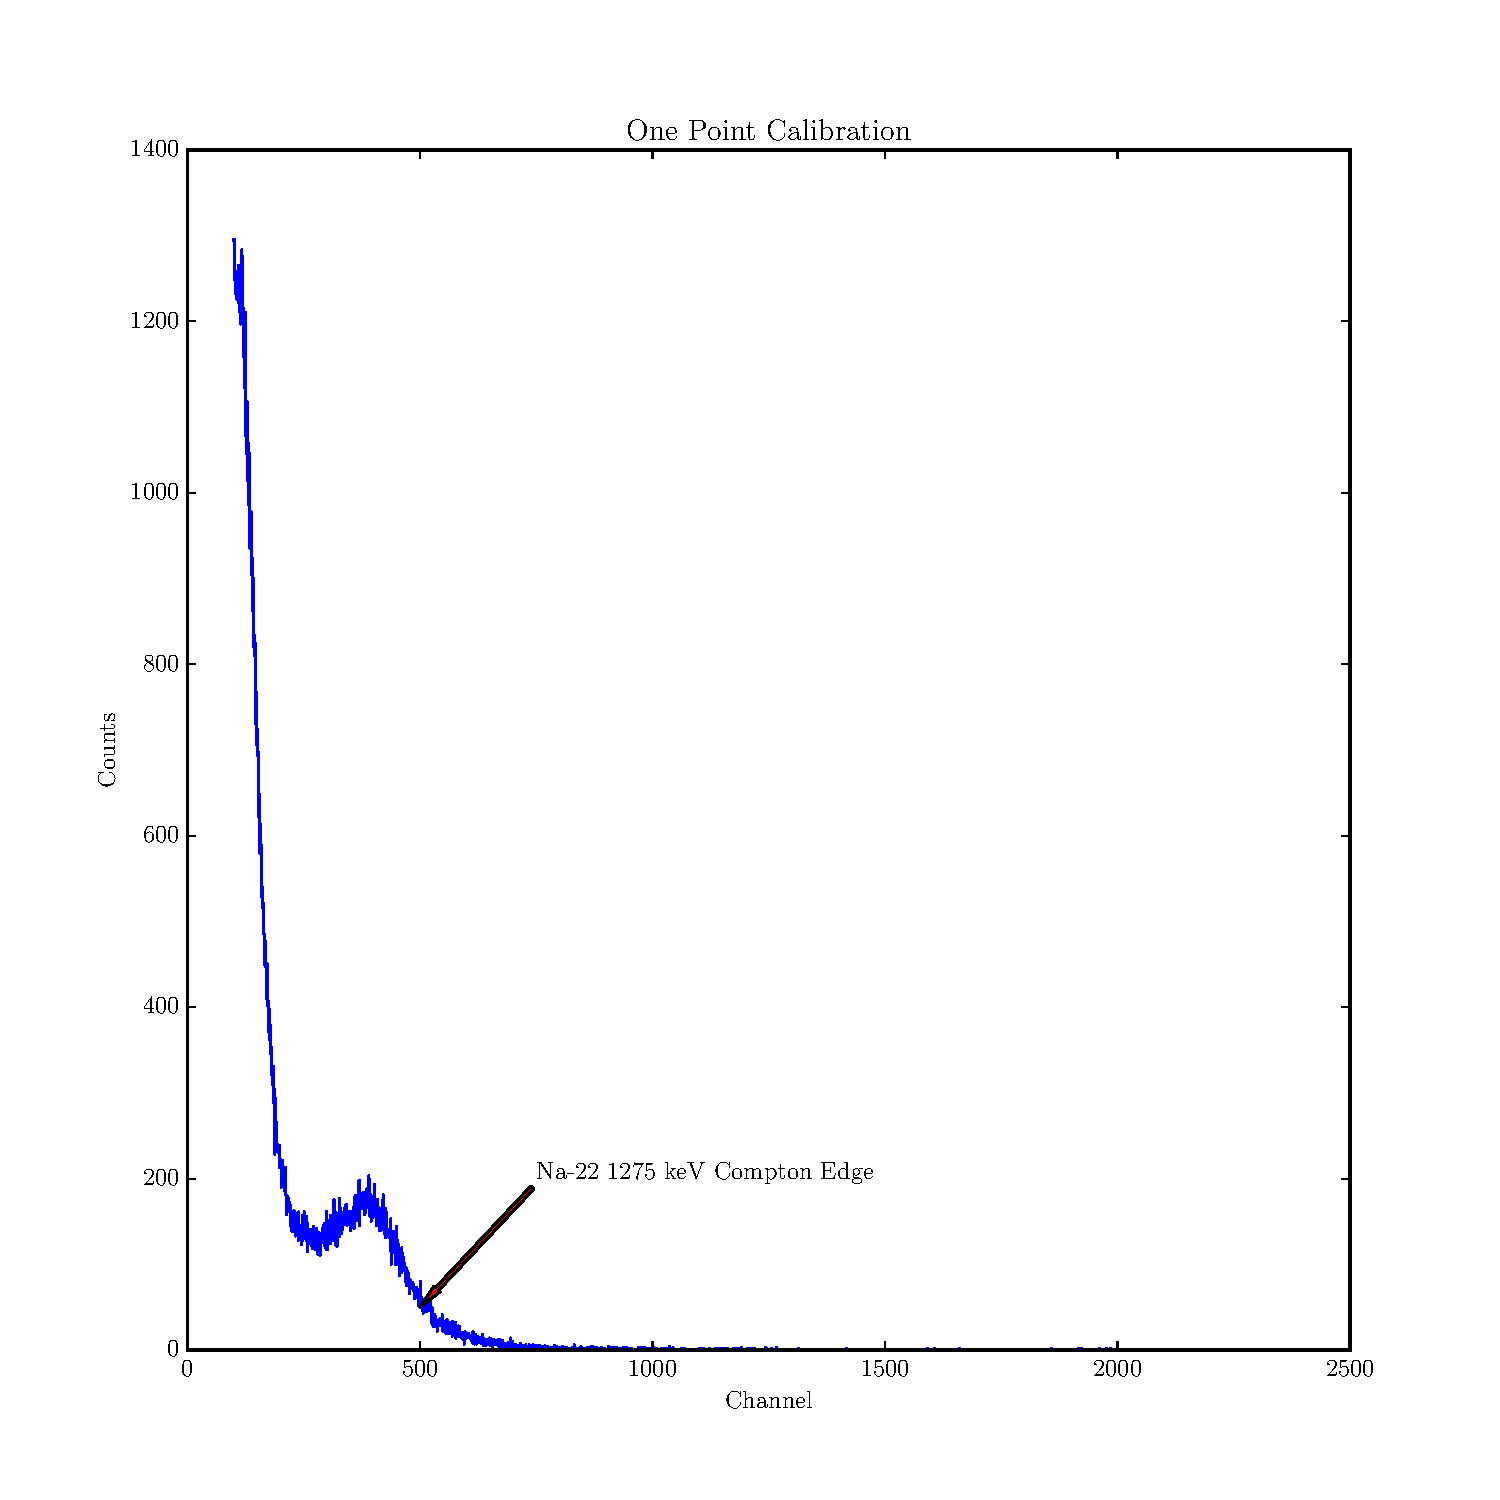
\includegraphics[scale=.4]{../plots/na_calibration_absorber_countrates.pdf} \\ 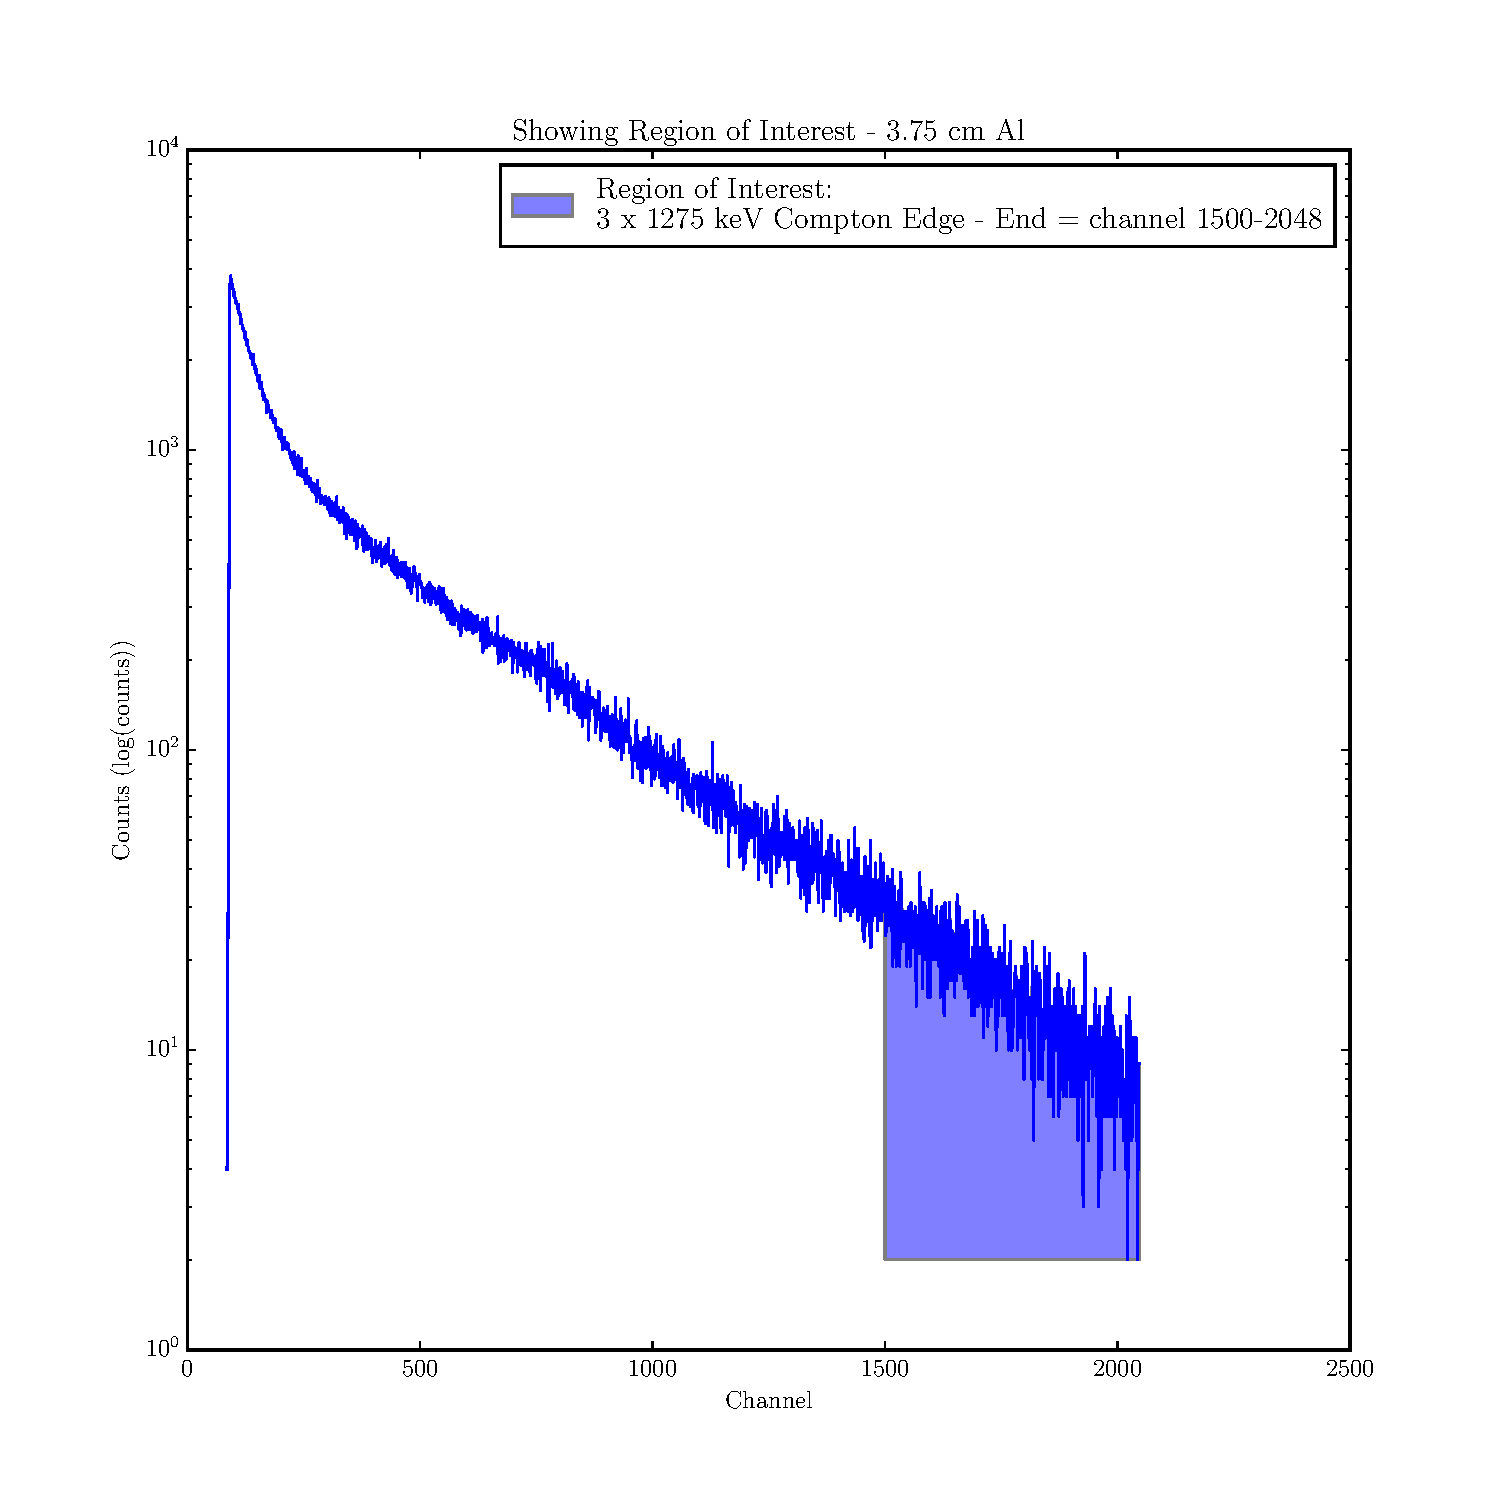
\includegraphics[scale=.4]{../plots/example_cross_section_highlight_roi.pdf}
    \end{tabular}
    \caption{Since the 1275 keV Compton edge is a rather broad feature, we choose one end, and a round number to make further calculations nicer.  Especially since the channels are integers, we cannot subdivide them and it is therefore beneficial to choose a nice round number that has a multiple of 3 in the integers.  Note that the plot that highlights the ROI is a semi-log plot in y so that we can better see the region of interest - as we can see from the Na-22 spectrum, one end tends to dominate if we don't show the counts axis in log scale.}
    \label{roi}
  \end{figure}

  \begin{figure}[!htb]
    \centering
    \begin{tabular}{c c}
      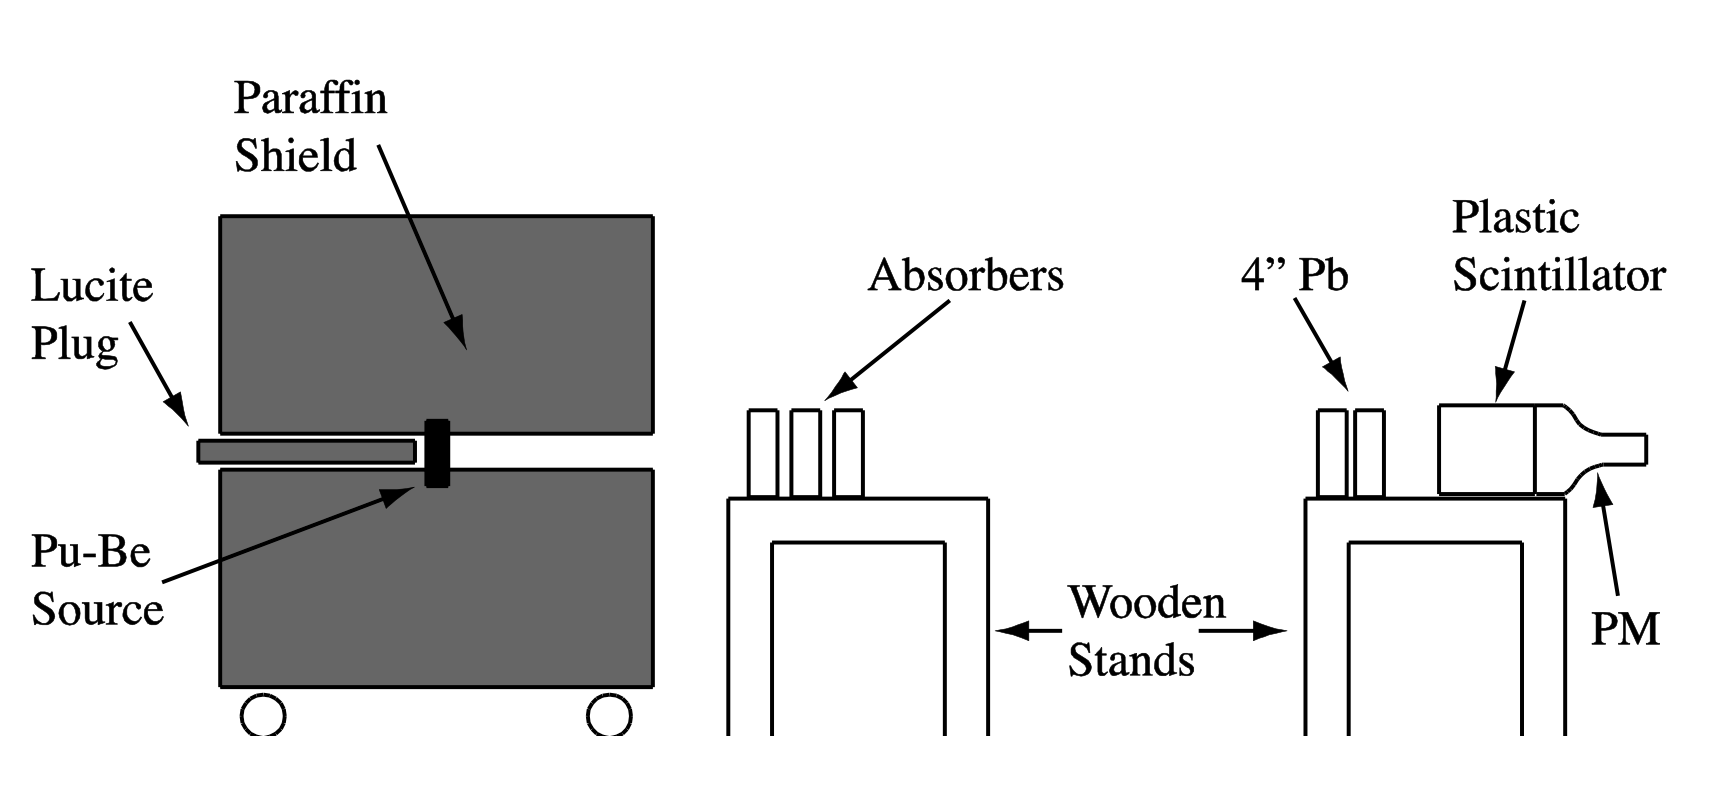
\includegraphics[scale=.25]{cross_section_apparatus.png} \\ 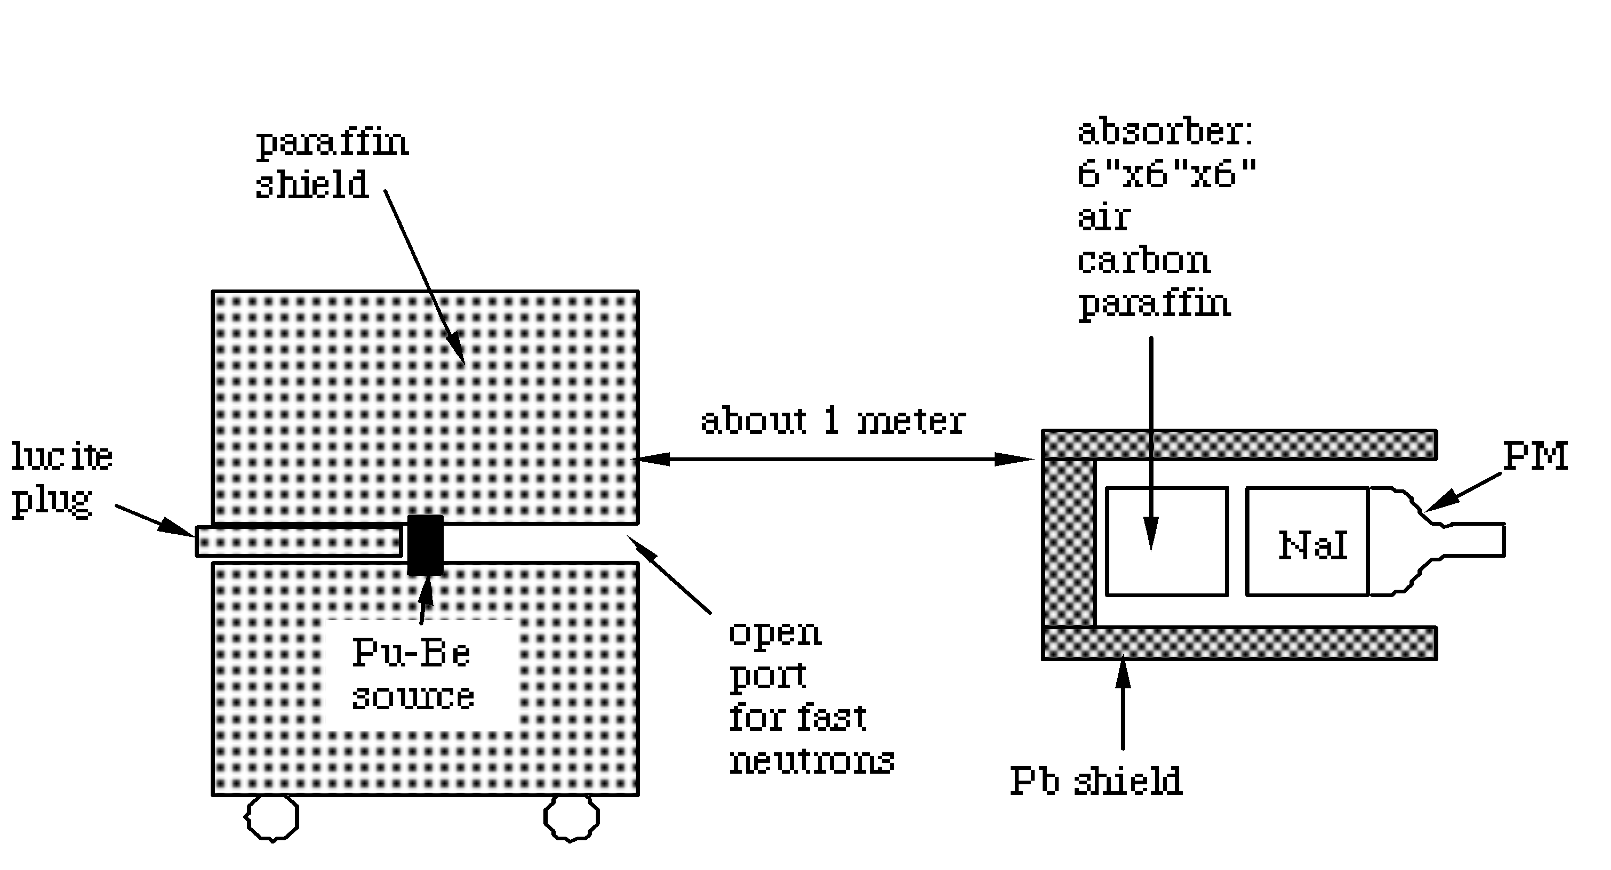
\includegraphics[scale=.25]{day_1_apparatus.png} \\
    \end{tabular}
    \caption{The top image is the experimental setup that we used to determine the radius of the neutron, the bottom image is the setup that allowed us to measure the capture photons from the deuteron reaction.  In reality, the wooden stand for the absorber was much closer to the detector for practicality reasons, but the essential setup is the same.}
    \label{apparatus}
  \end{figure}

  \begin{figure}[!htb]
    \centering
    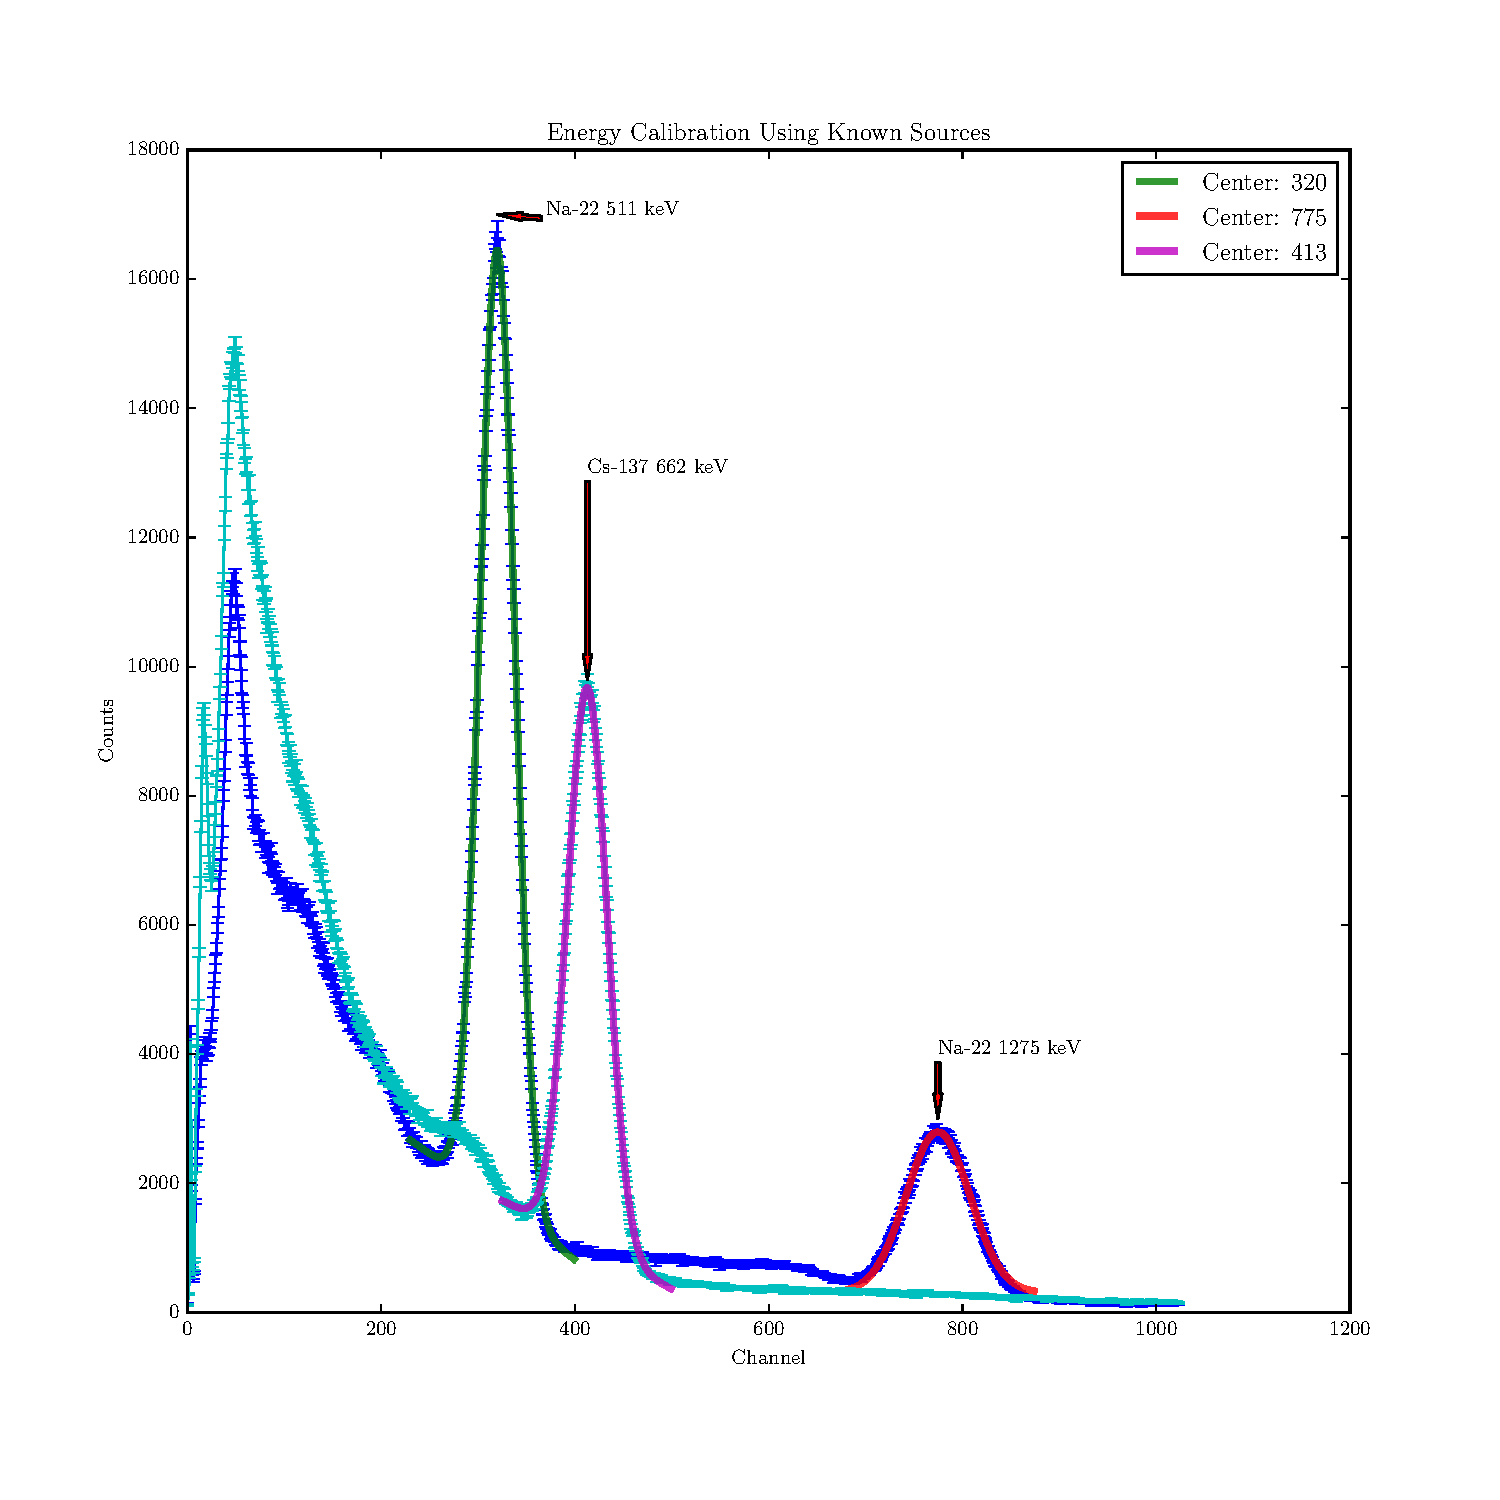
\includegraphics[scale=.5]{../plots/calibration_peaks.pdf}
    \caption{Peaks are labeled on the plot itself, and the centers are cited as well.  It is clear that the centers are known to within better than 1 channel.  The 3 peaks were fit to the form $f(x) = Ae^{\frac{-(x-\mu)^2}{2\sigma^2}} + Bx + C.$ The \redchi values of the three peaks are, from left to right, 1.96, 2.14, and 4.62.  These values indicate good fits, and this is also reflected in the uncertainty for the peak centers.}
    \label{cal_peaks}
  \end{figure}

  \begin{figure}[!htb]
    \centering
    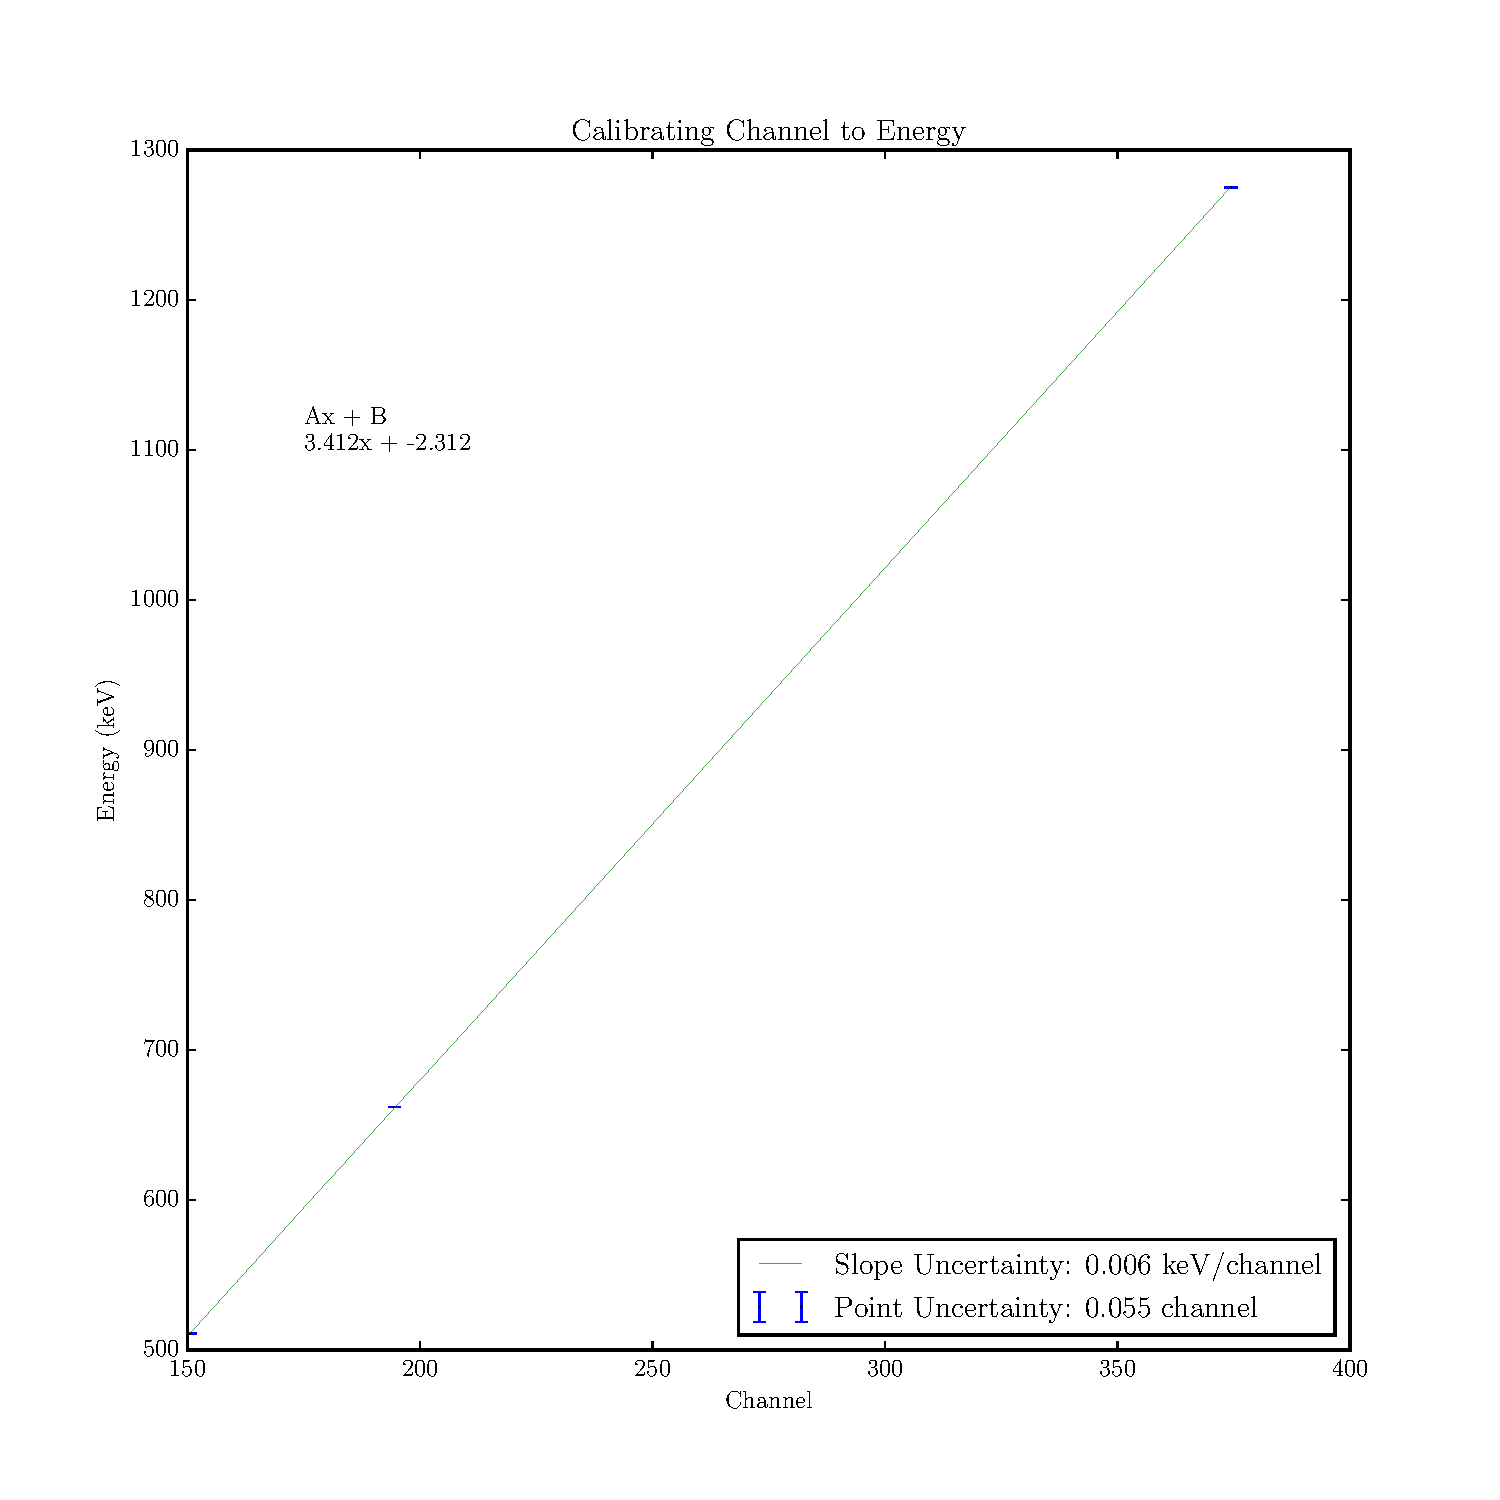
\includegraphics[scale=.5]{../plots/channel_energy_cal.pdf}
    \caption{The \redchi value for this line is 0.94, almost a perfect fit.  The uncertainty in the slope is noted on the plot itself, it is 0.006 kev/channel.  The uncertainty in the intercept is the same as the point uncertainty quoted as 0.055 channel.  This corresponds to approximately 0.17 keV, or less than 0.04\% of the lowest measurement.  Since we will be making measurements at the 2000 keV range, this uncertainty is less than 0.01\%.}
    \label{calibration}
  \end{figure}

  \begin{figure}[!htb]
    \centering
    \begin{tabular}{c c}
      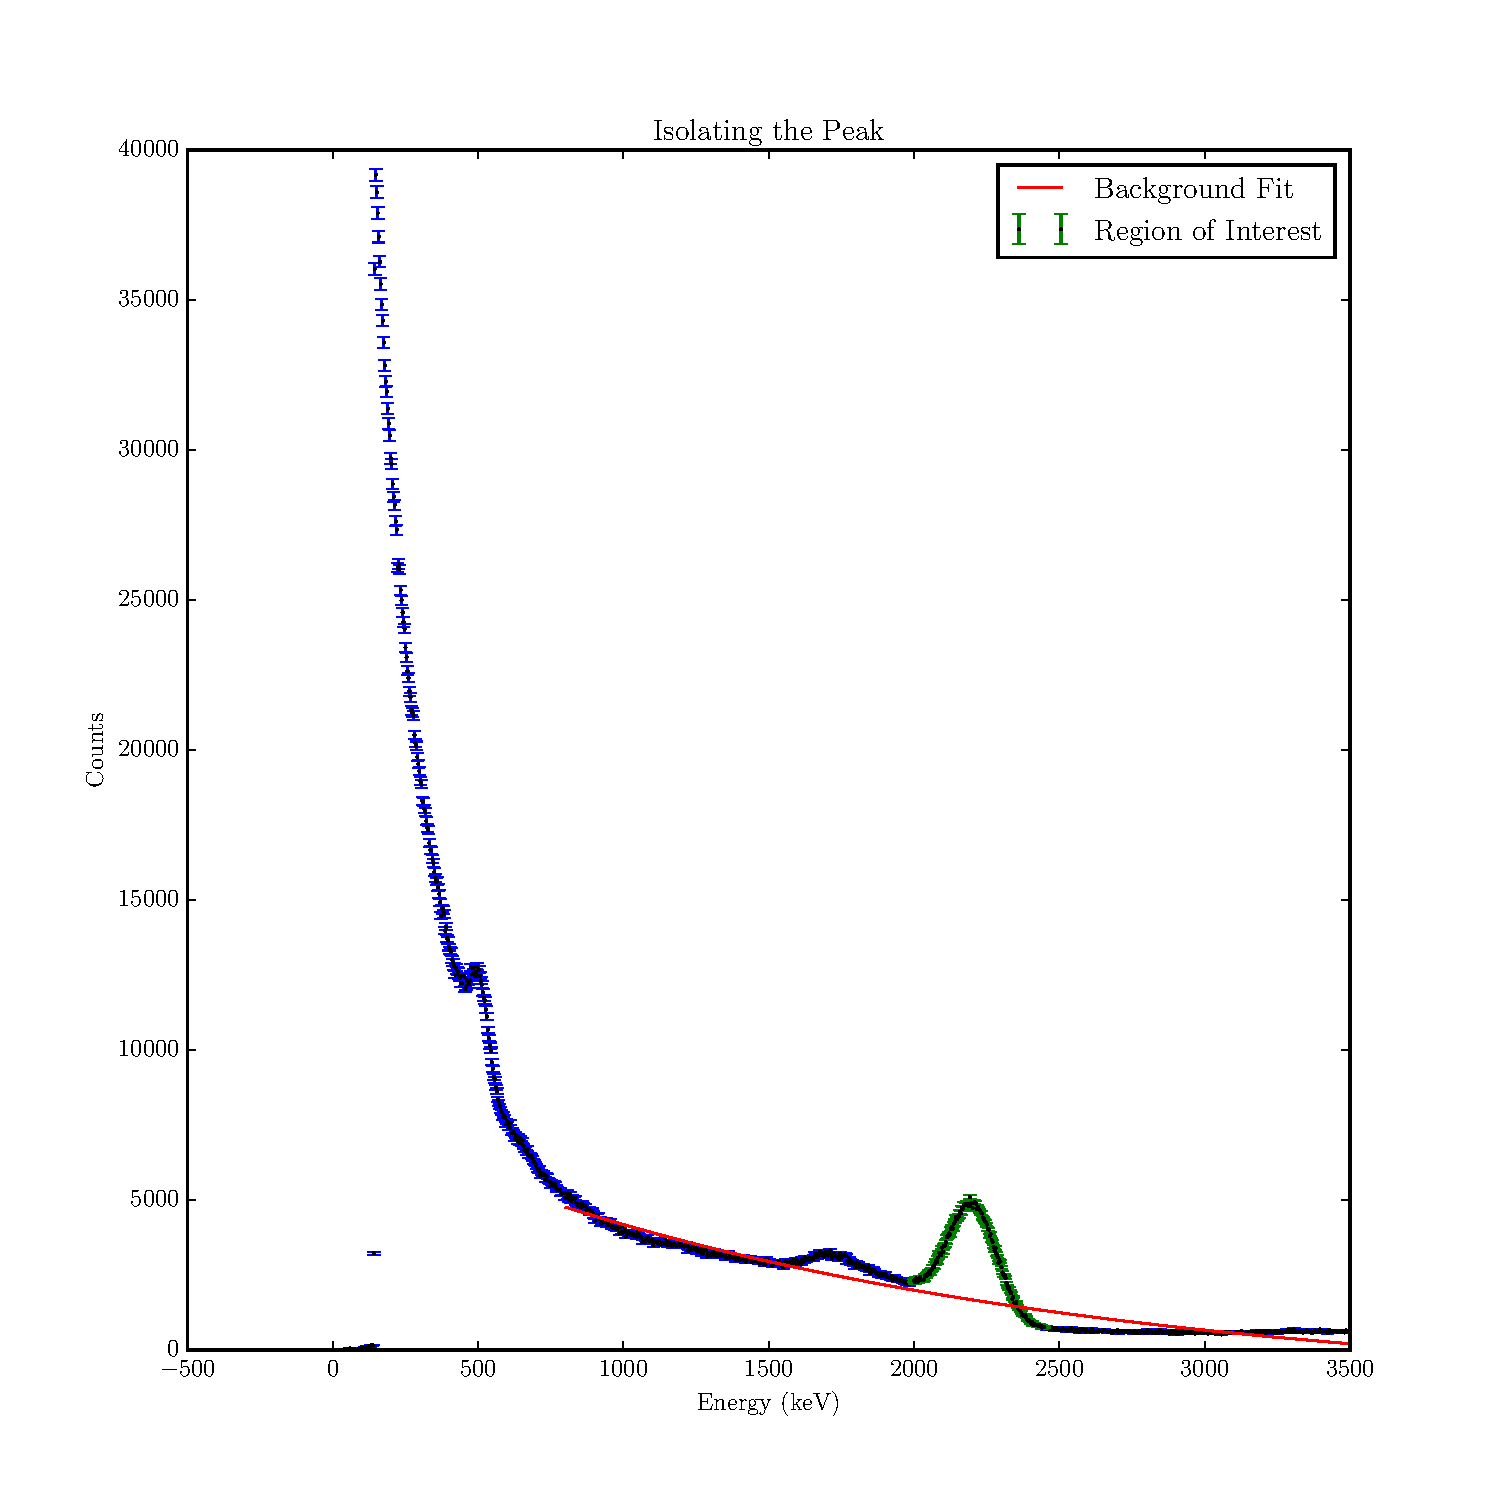
\includegraphics[width=.5\linewidth]{../plots/peak_isolation_nolead_portclosed.pdf} & 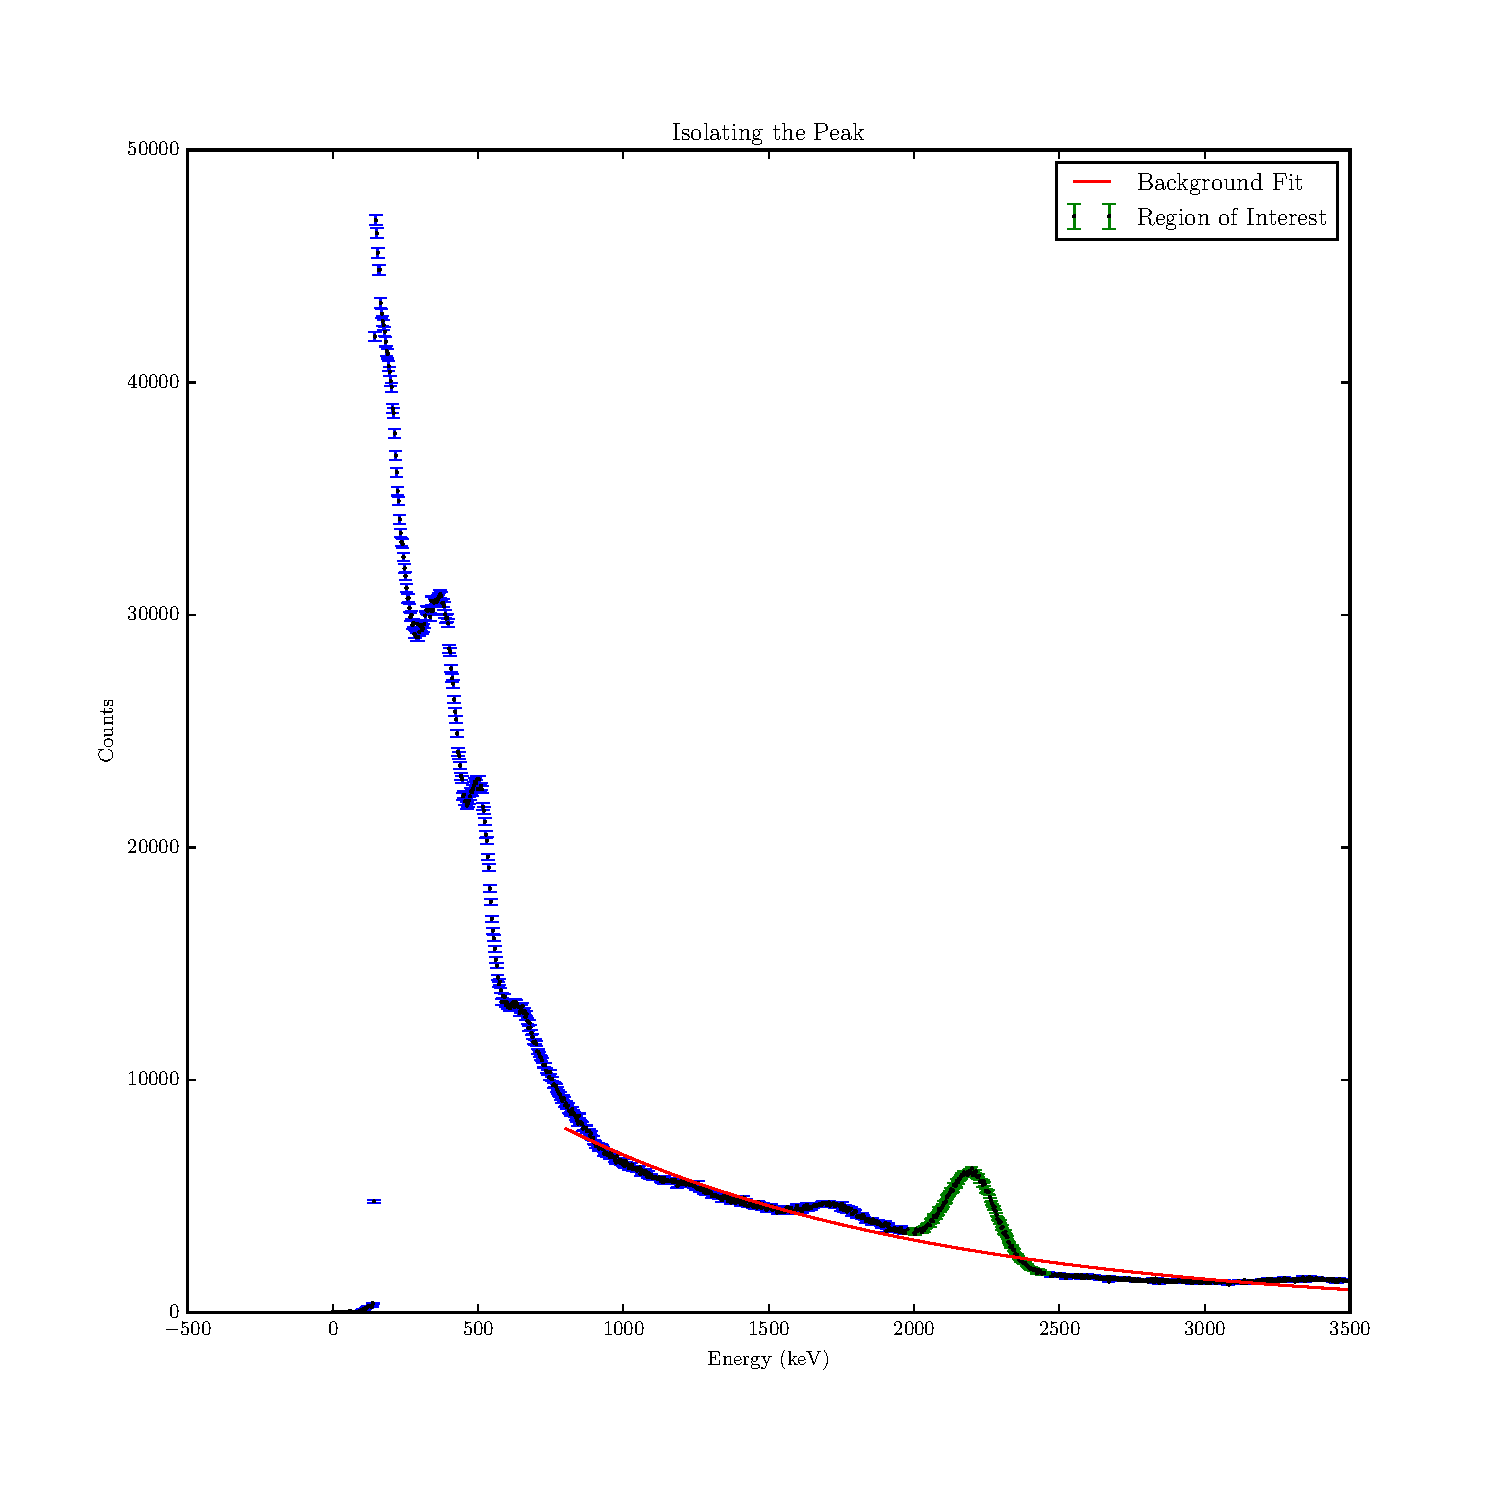
\includegraphics[width=.5\linewidth]{../plots/peak_isolation_nolead_portopen.pdf} \\
      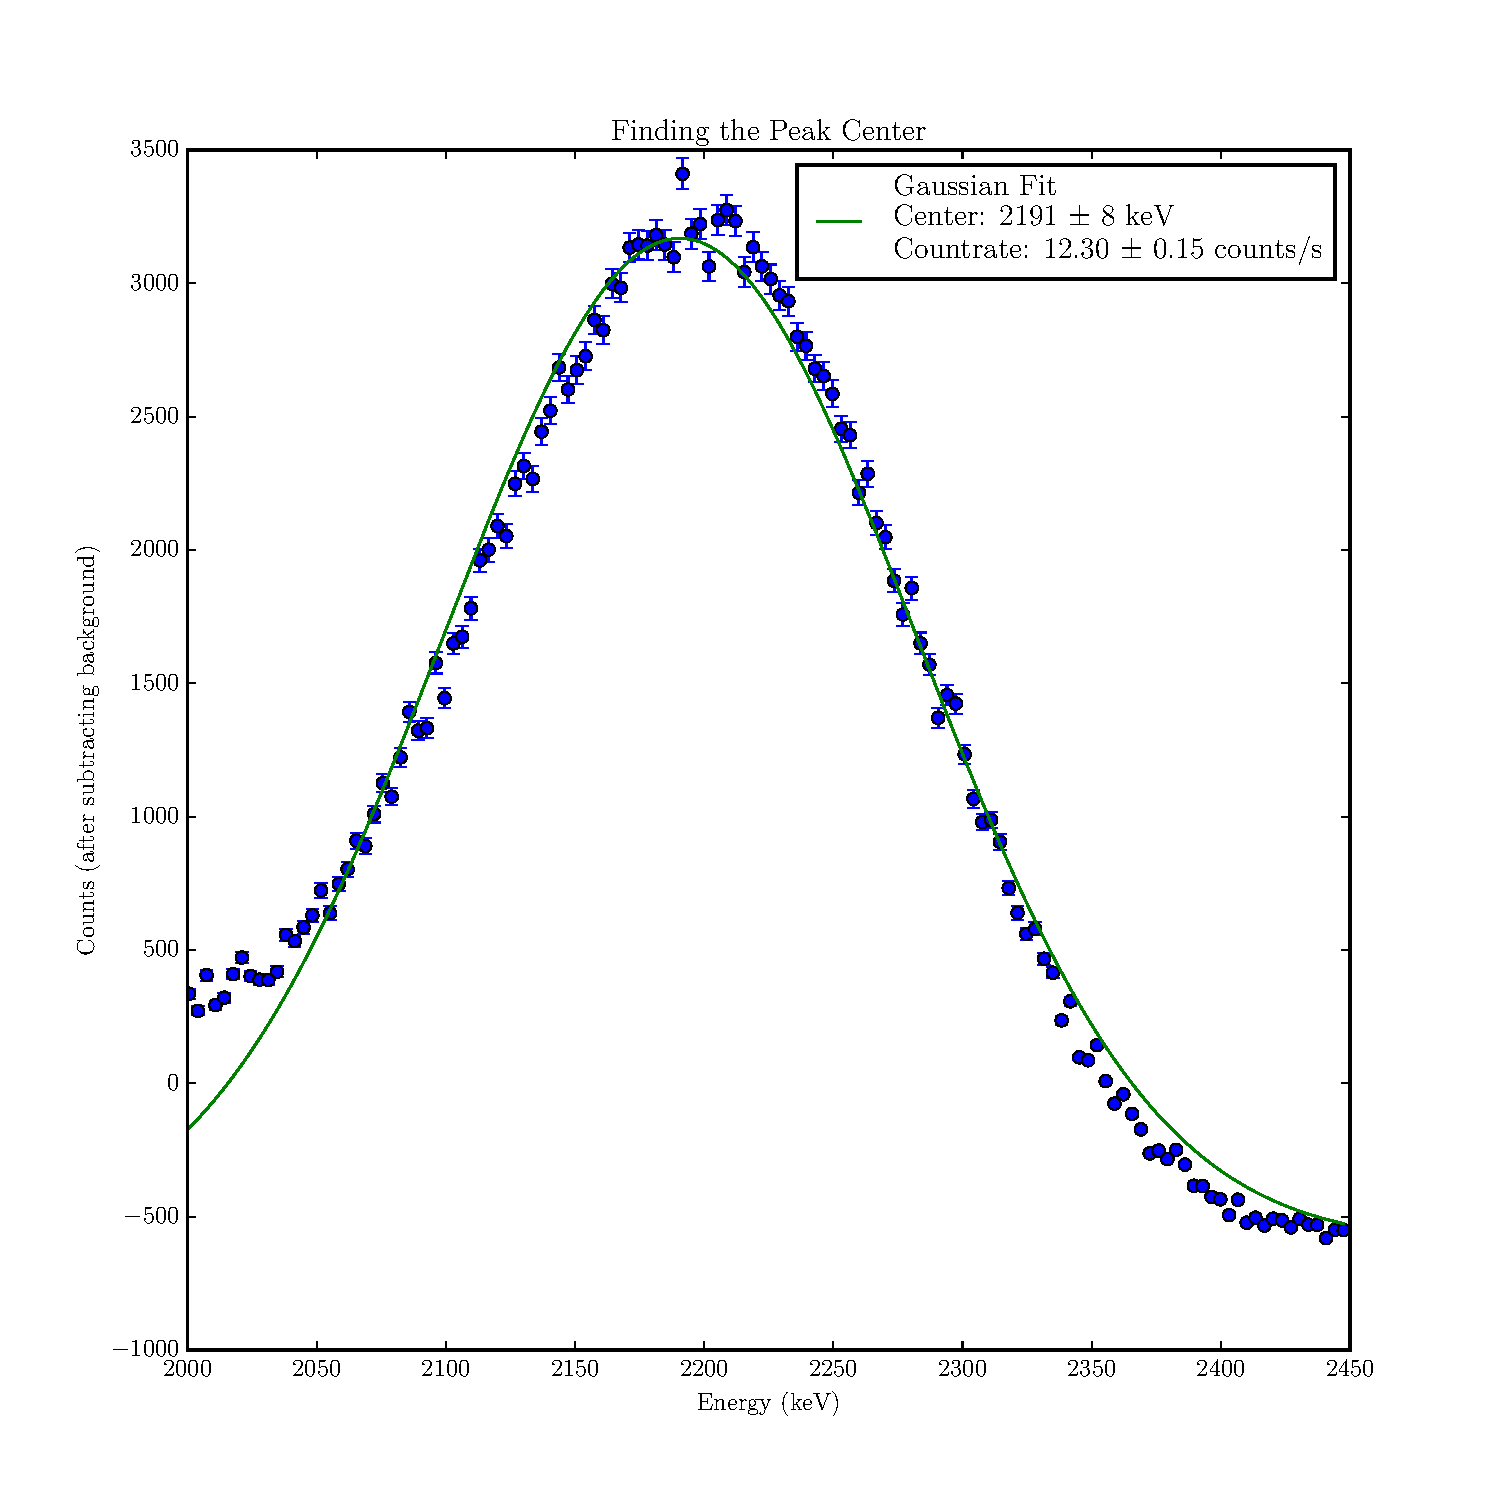
\includegraphics[width=.5\linewidth]{../plots/peak_center_nolead_portclosed.pdf} & 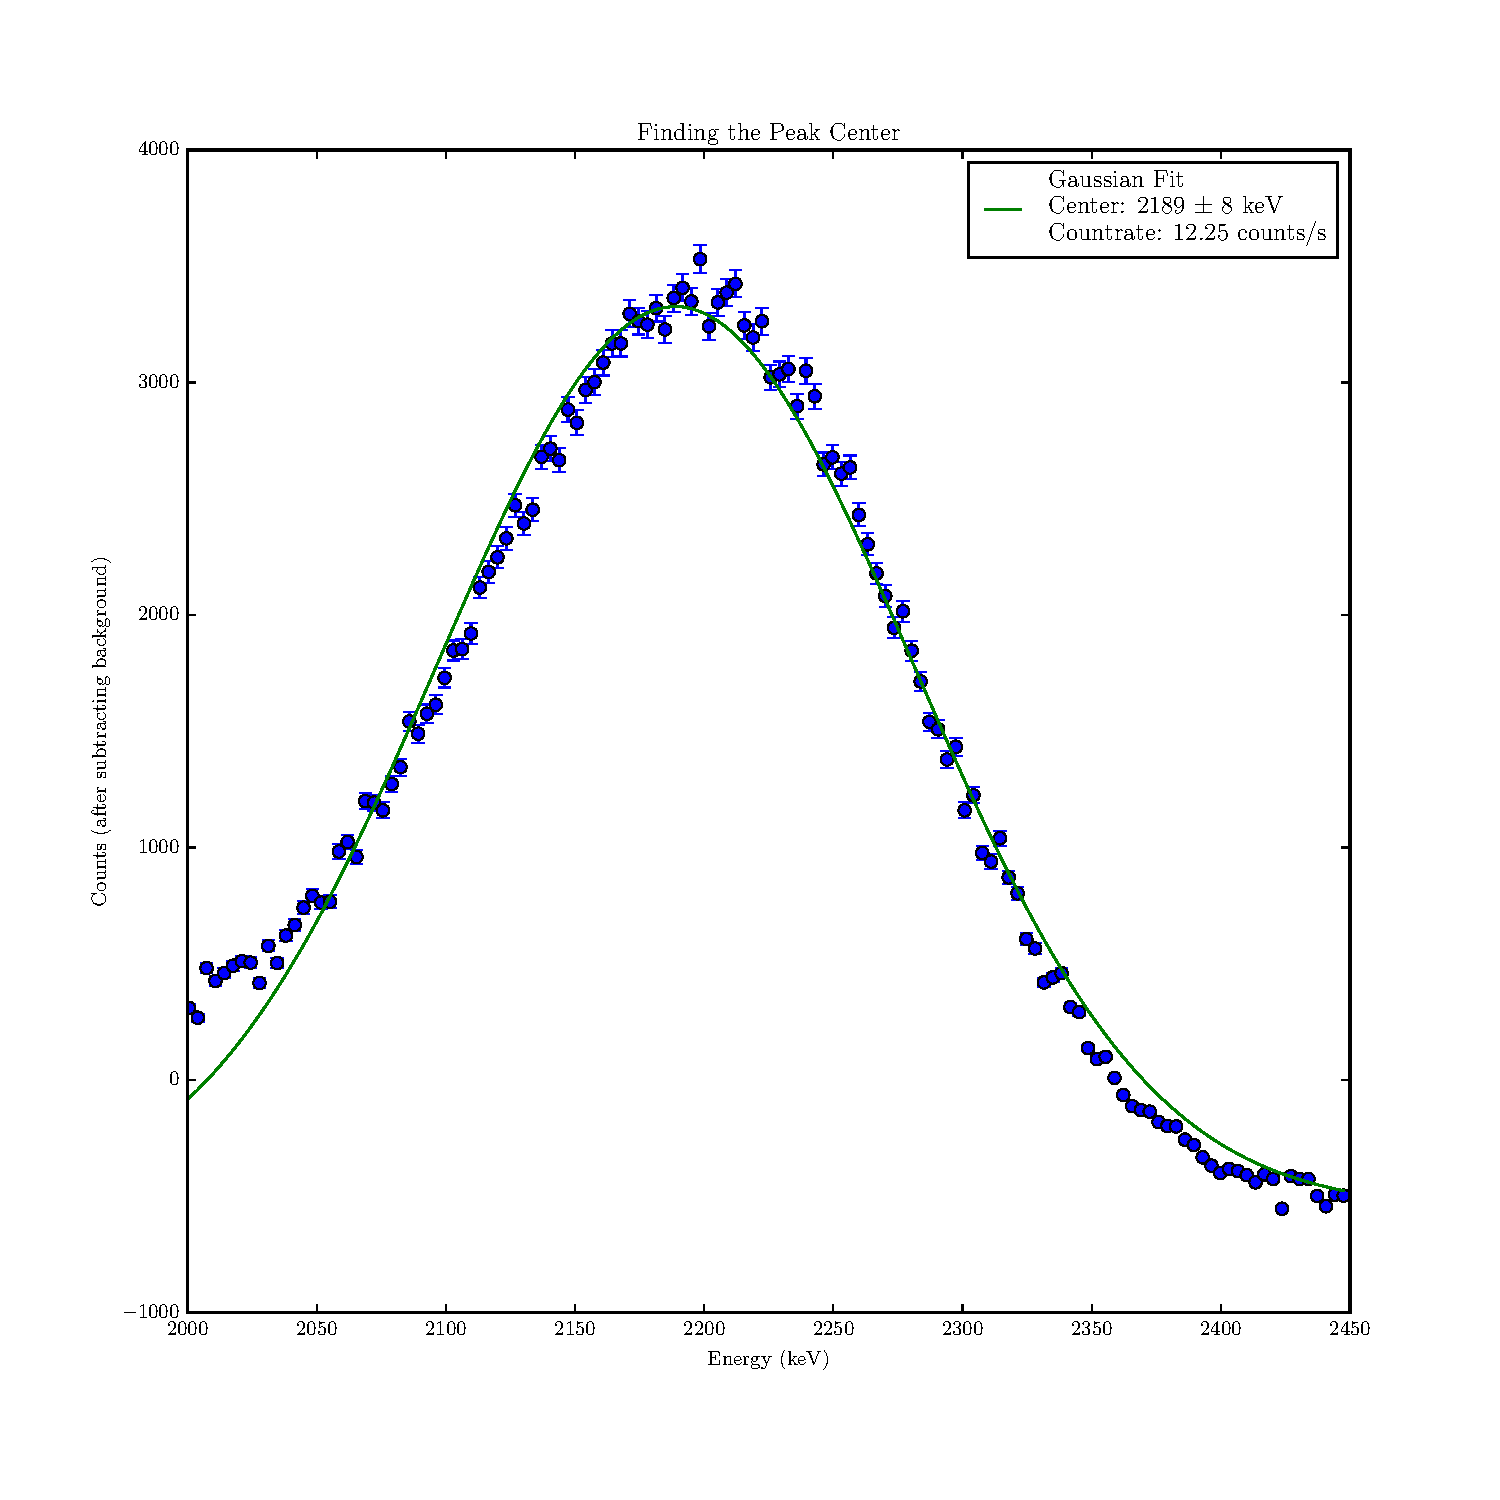
\includegraphics[width=.5\linewidth]{../plots/peak_center_nolead_portopen.pdf} \\
    \end{tabular}
    \caption{The background fit was a simple decaying exponential, $f(x) = Ae^{-Bx} + C$.  In both cases the \redchi value was not stellar (from left to right, 26.45 and 27.87) but we are not necessarily looking for a perfect fit in this instance, we only need to verify the peak center (to make sure we are measuring the right feature) and amplitude to find the countrate, which is the amplitude of the Gaussian fit perfomed on the two bottom peaks divided by the livetime.  The bottom two peaks are zoomed in plots of the green regions on the top two plots, and each peak corresponds to the plot directly above it.  The \redchi values for the bottom two peaks are 13.23 and 14.54 from left to right.  Again, not stellar but we can visually confirm that the fits are good enough for our purposes.}
    \label{nolead}
  \end{figure}

  \begin{figure}[!htb]
    \centering
    \begin{tabular}{c c}
      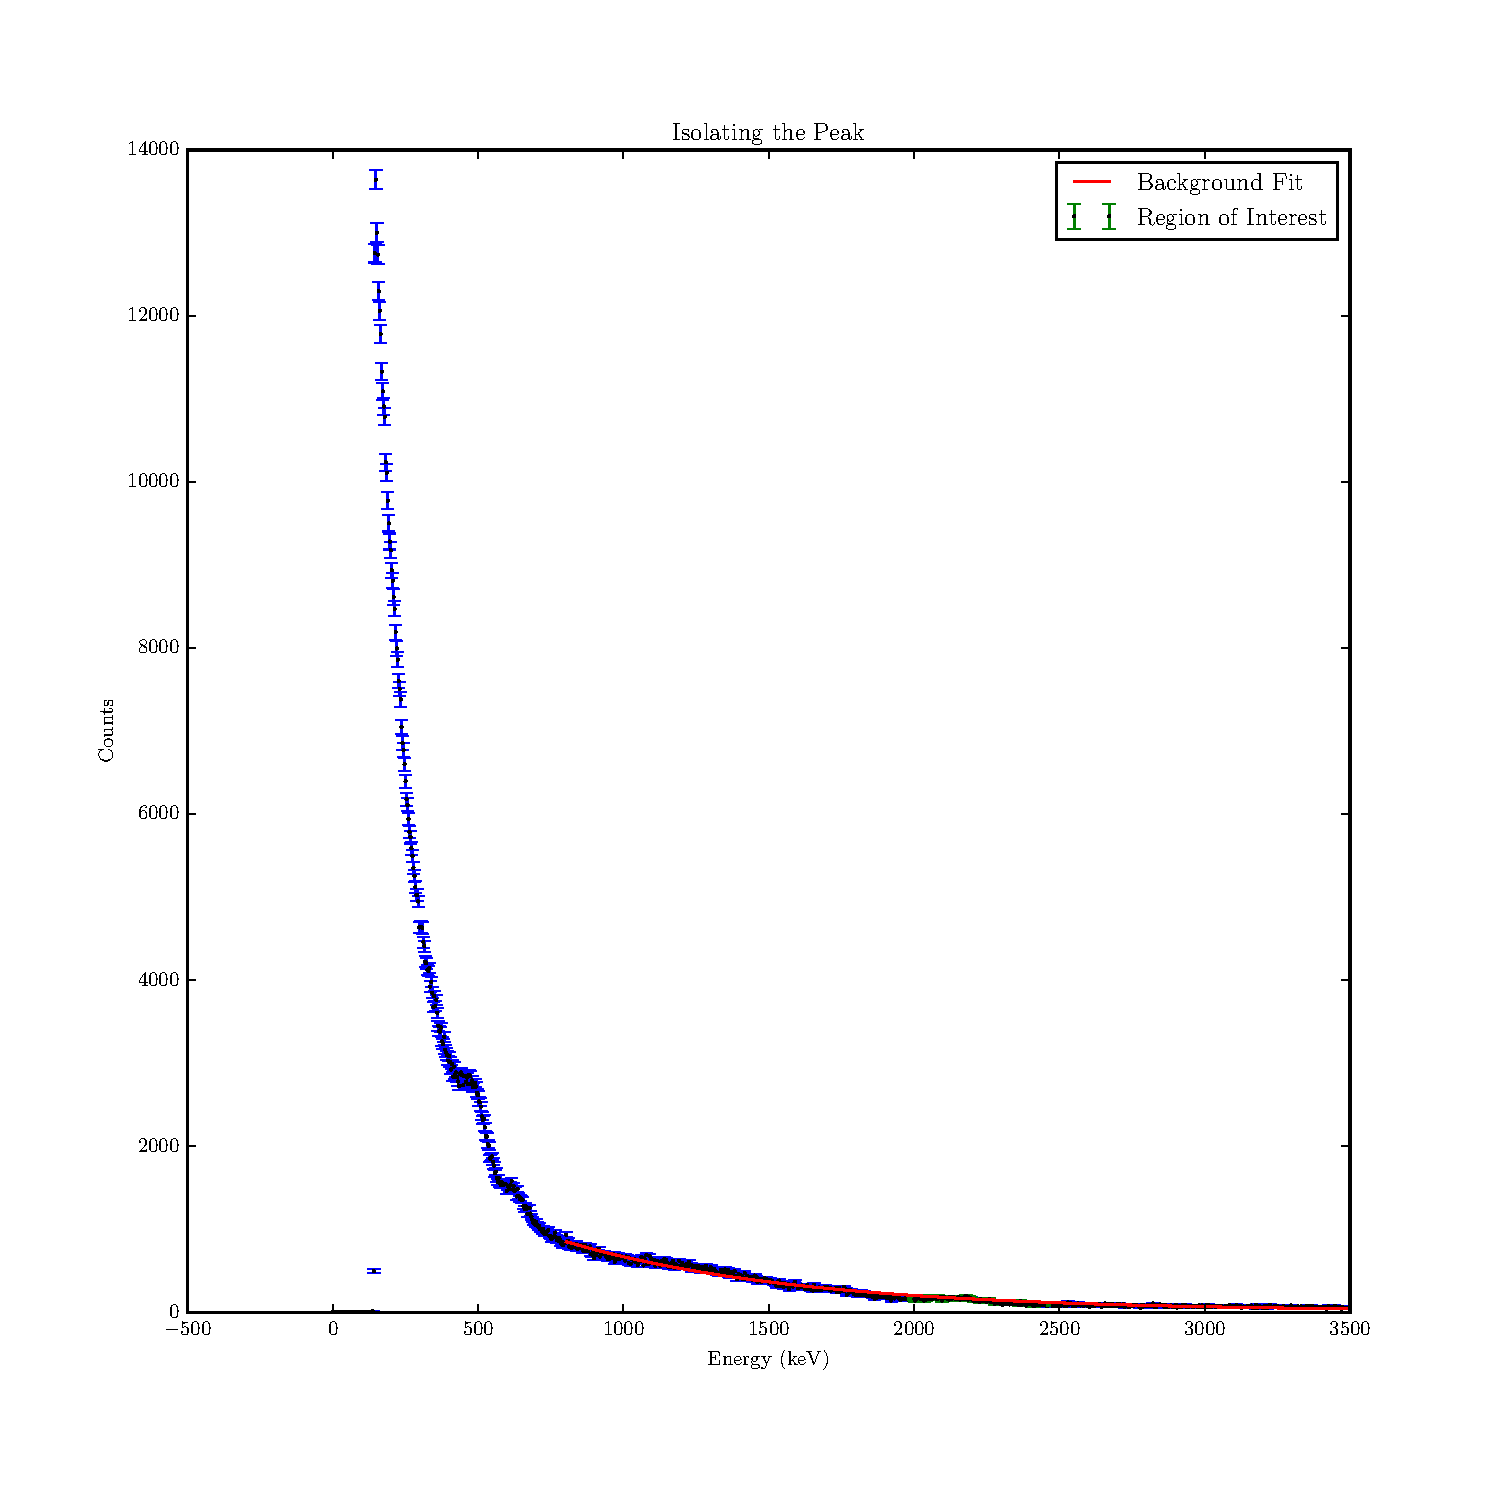
\includegraphics[width=.5\linewidth]{../plots/peak_isolation_lead_portclosed.pdf} & 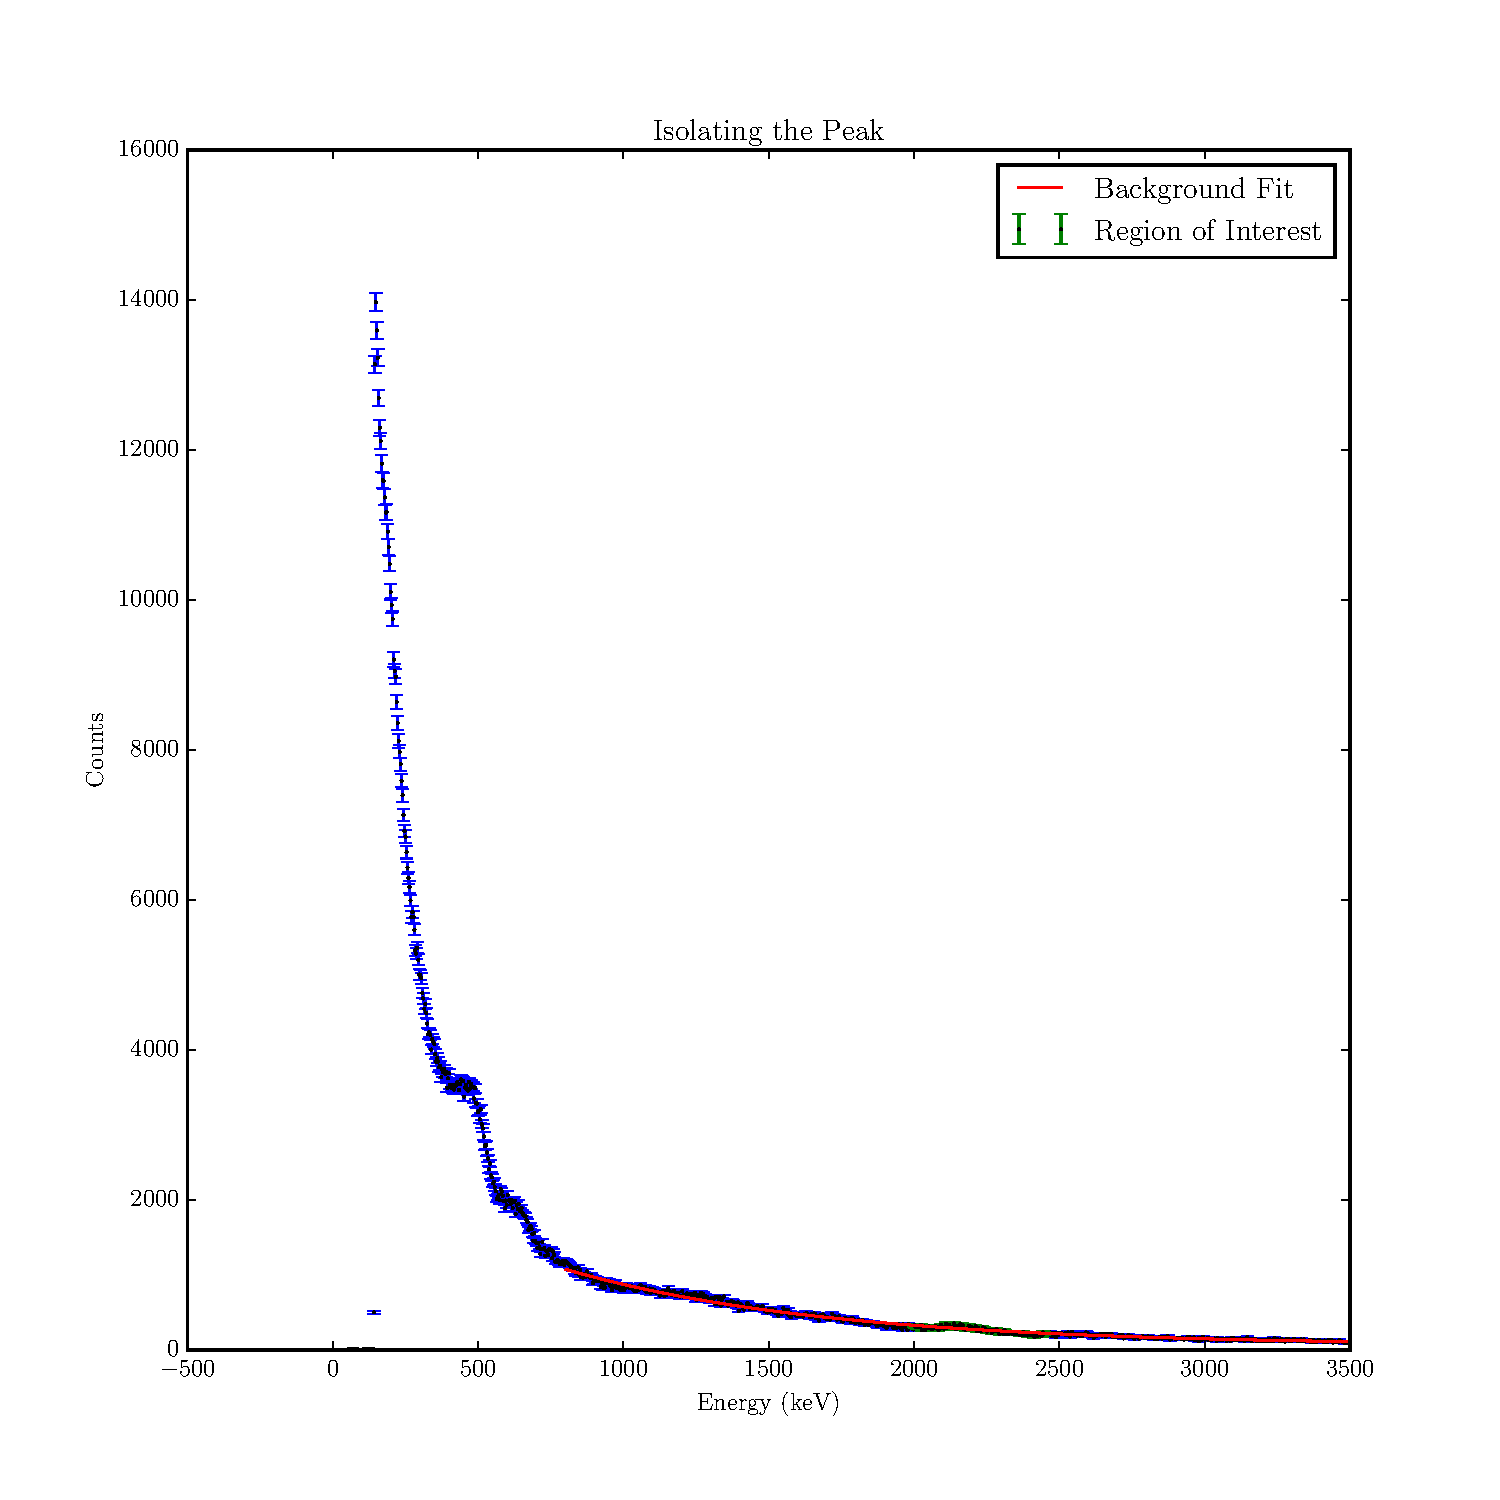
\includegraphics[width=.5\linewidth]{../plots/peak_isolation_lead_portopen.pdf} \\
      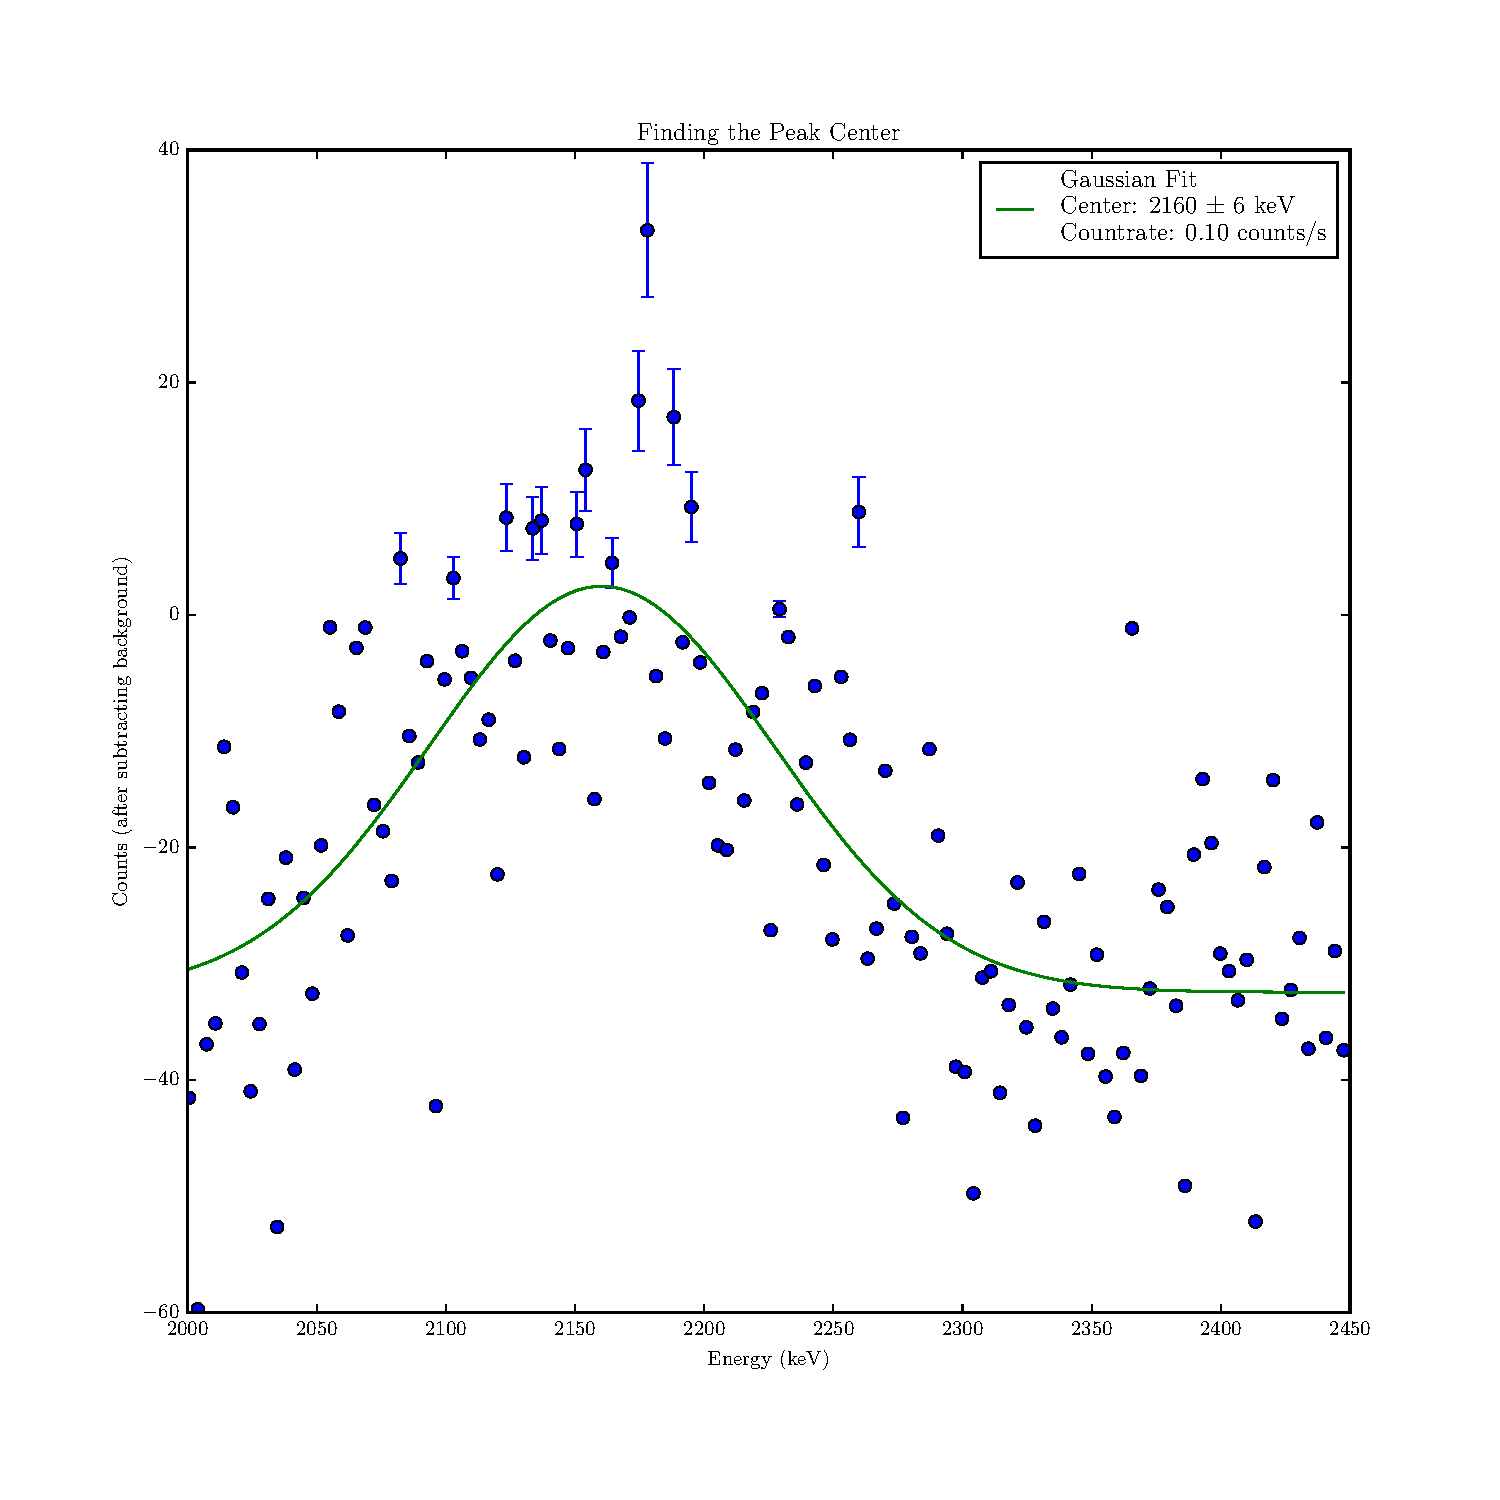
\includegraphics[width=.5\linewidth]{../plots/peak_center_lead_portclosed.pdf} & 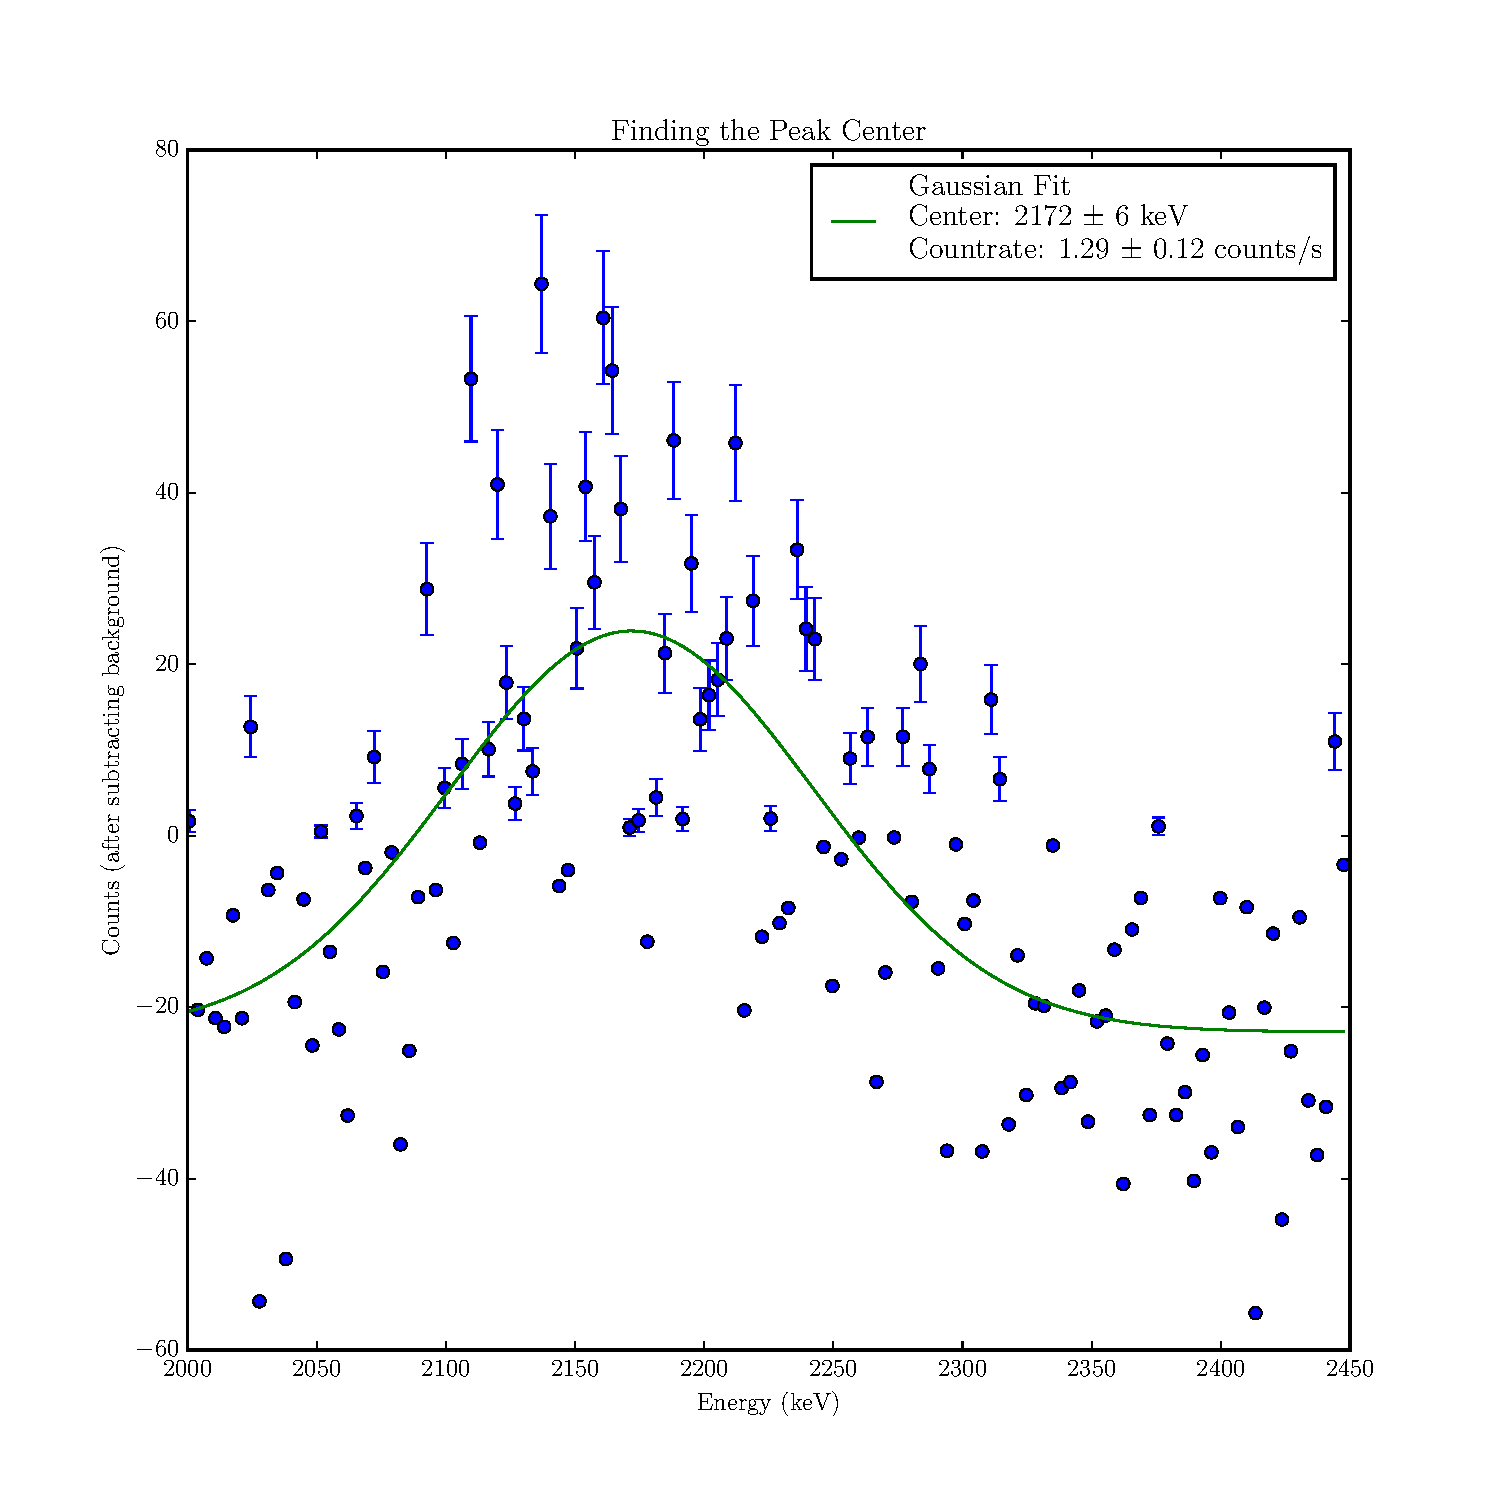
\includegraphics[width=.5\linewidth]{../plots/peak_center_lead_portopen.pdf} \\
    \end{tabular}
    \caption{The background fit on the top two plots had a much better \redchi value, 3.86 and 4.21 from left to right, but it's nearly meaningless because as we can see on the bottom two plots, the countrates have a 10\% uncertainty, and from the \redchi values (176.33 and 186.19) we know that the fits mean very little aside from giving us a baseline for what will give us roughly zero, and even that is barely meaningful.}
    \label{lead}
  \end{figure}

  \begin{figure}[!htb]
    \centering
    \begin{tabular}{c c}
      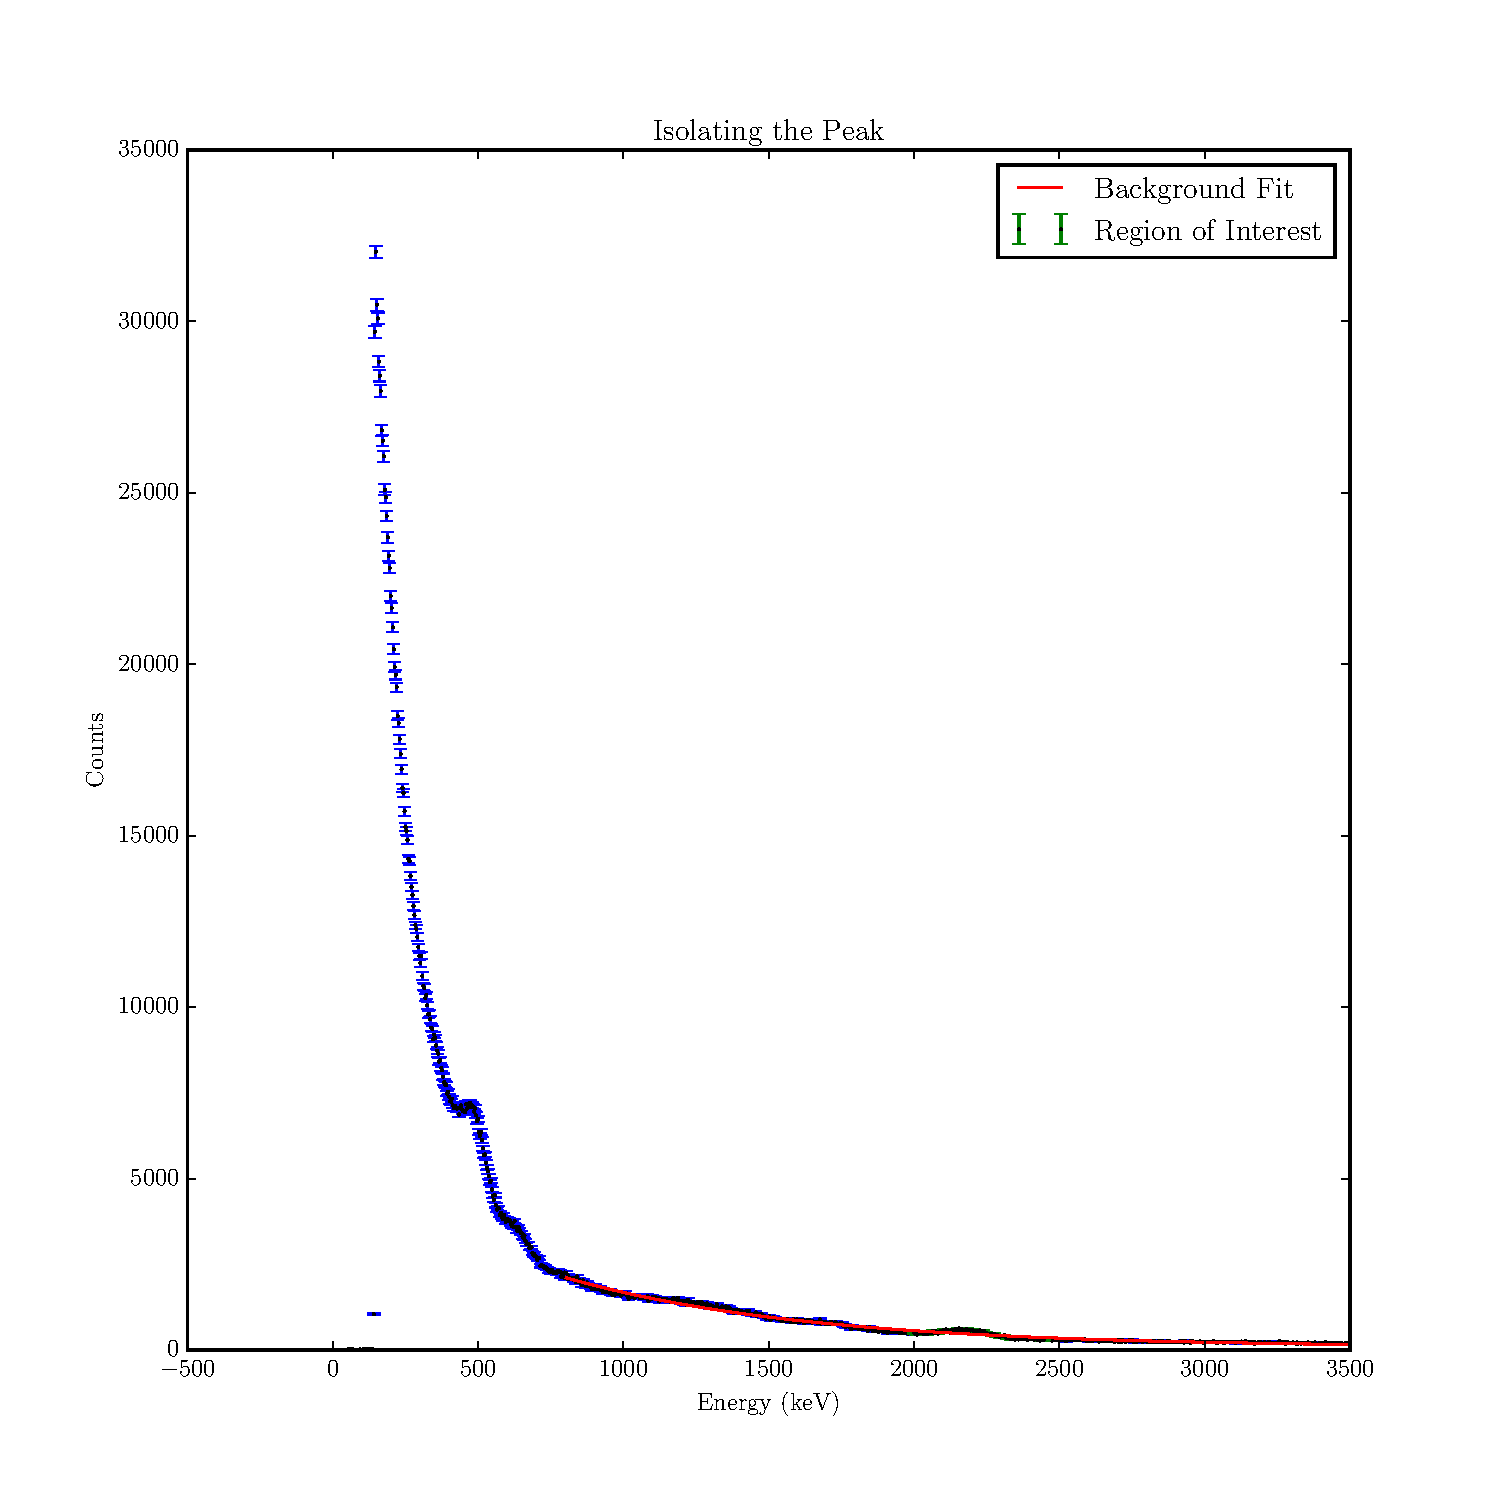
\includegraphics[scale=.4]{../plots/peak_isolation_shielded_paraffin.pdf} \\ 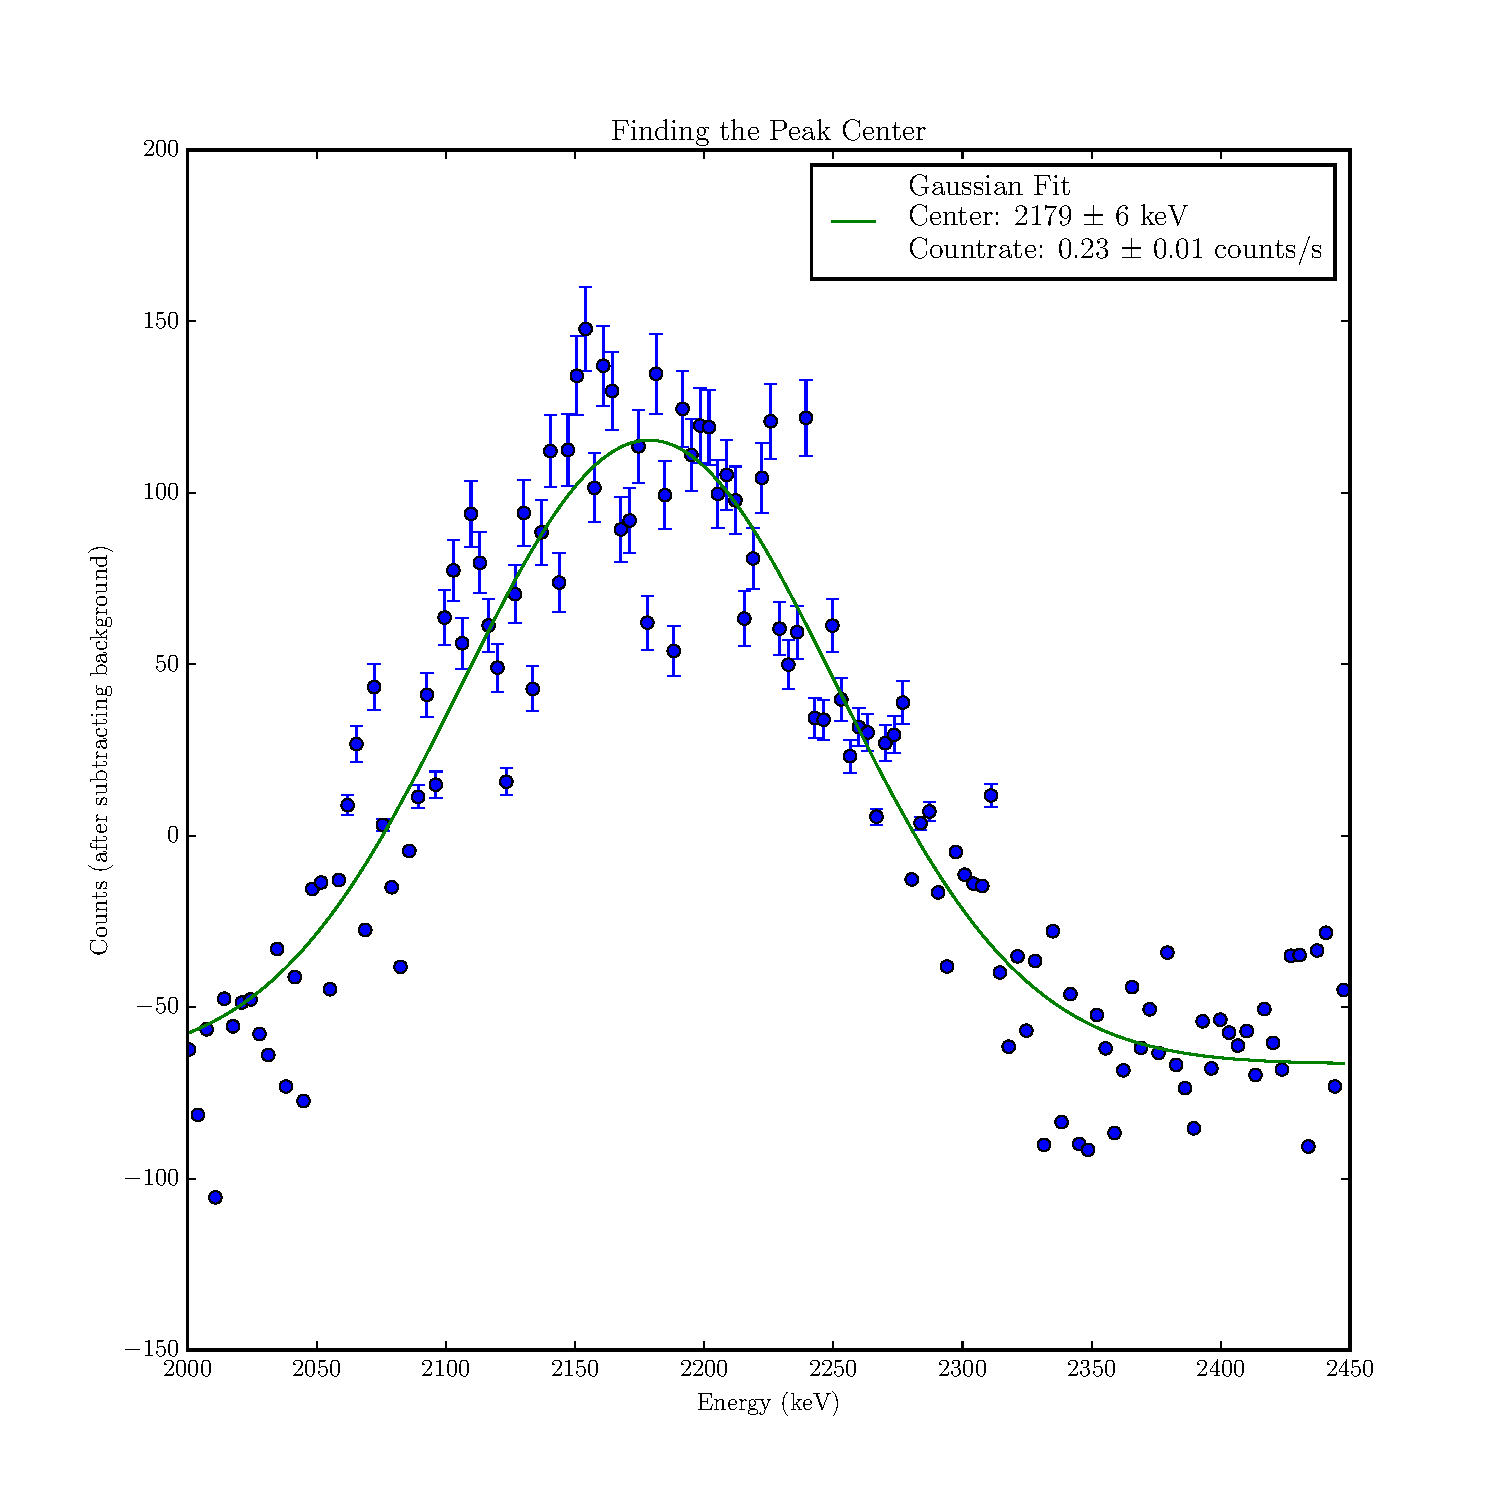
\includegraphics[scale=.4]{../plots/peak_center_shielded_paraffin.pdf} \\
    \end{tabular}
    \caption{A very small peak to be sure, but a peak nonetheless.  Importantly we note the uncertainty on the countrate - the reported countrate is \textbf{not} within uncertainties of zero.  The \redchi value is surprisingly good, it is 28.31 which can be explained by the fact that the data is well-spread about the fitted curve, although it is plausible that the fitted curve describes the mean of the data.  Furthermore, in this case (and others) when the values are below 0 from subtracting the background, the uncertainty is ill-defined and as such the \redchi value is inflated artificially.}
    \label{paraffin}
  \end{figure}

  \begin{figure}[!htb]
    \centering
    \begin{tabular}{c c}
      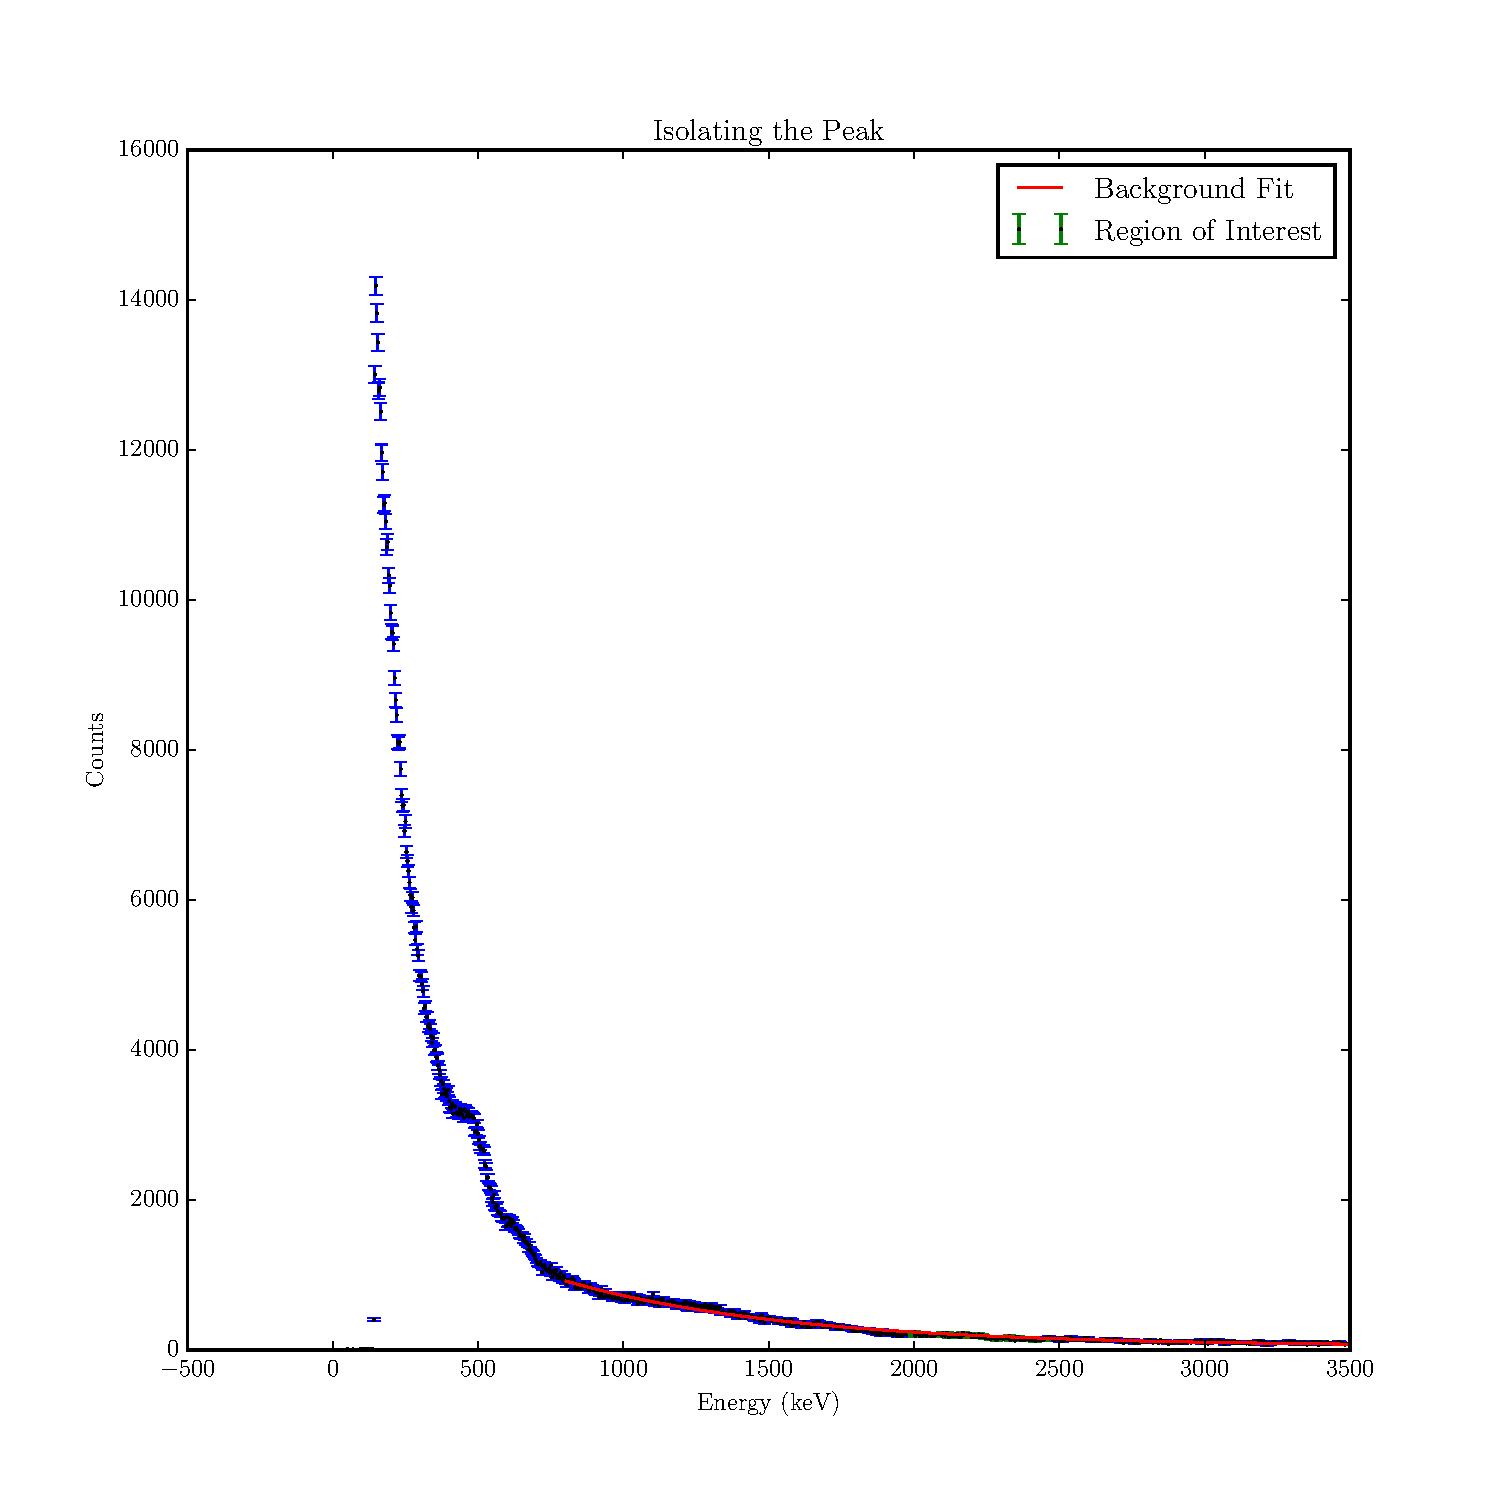
\includegraphics[scale=.4]{../plots/peak_isolation_shielded_carbon.pdf} \\ 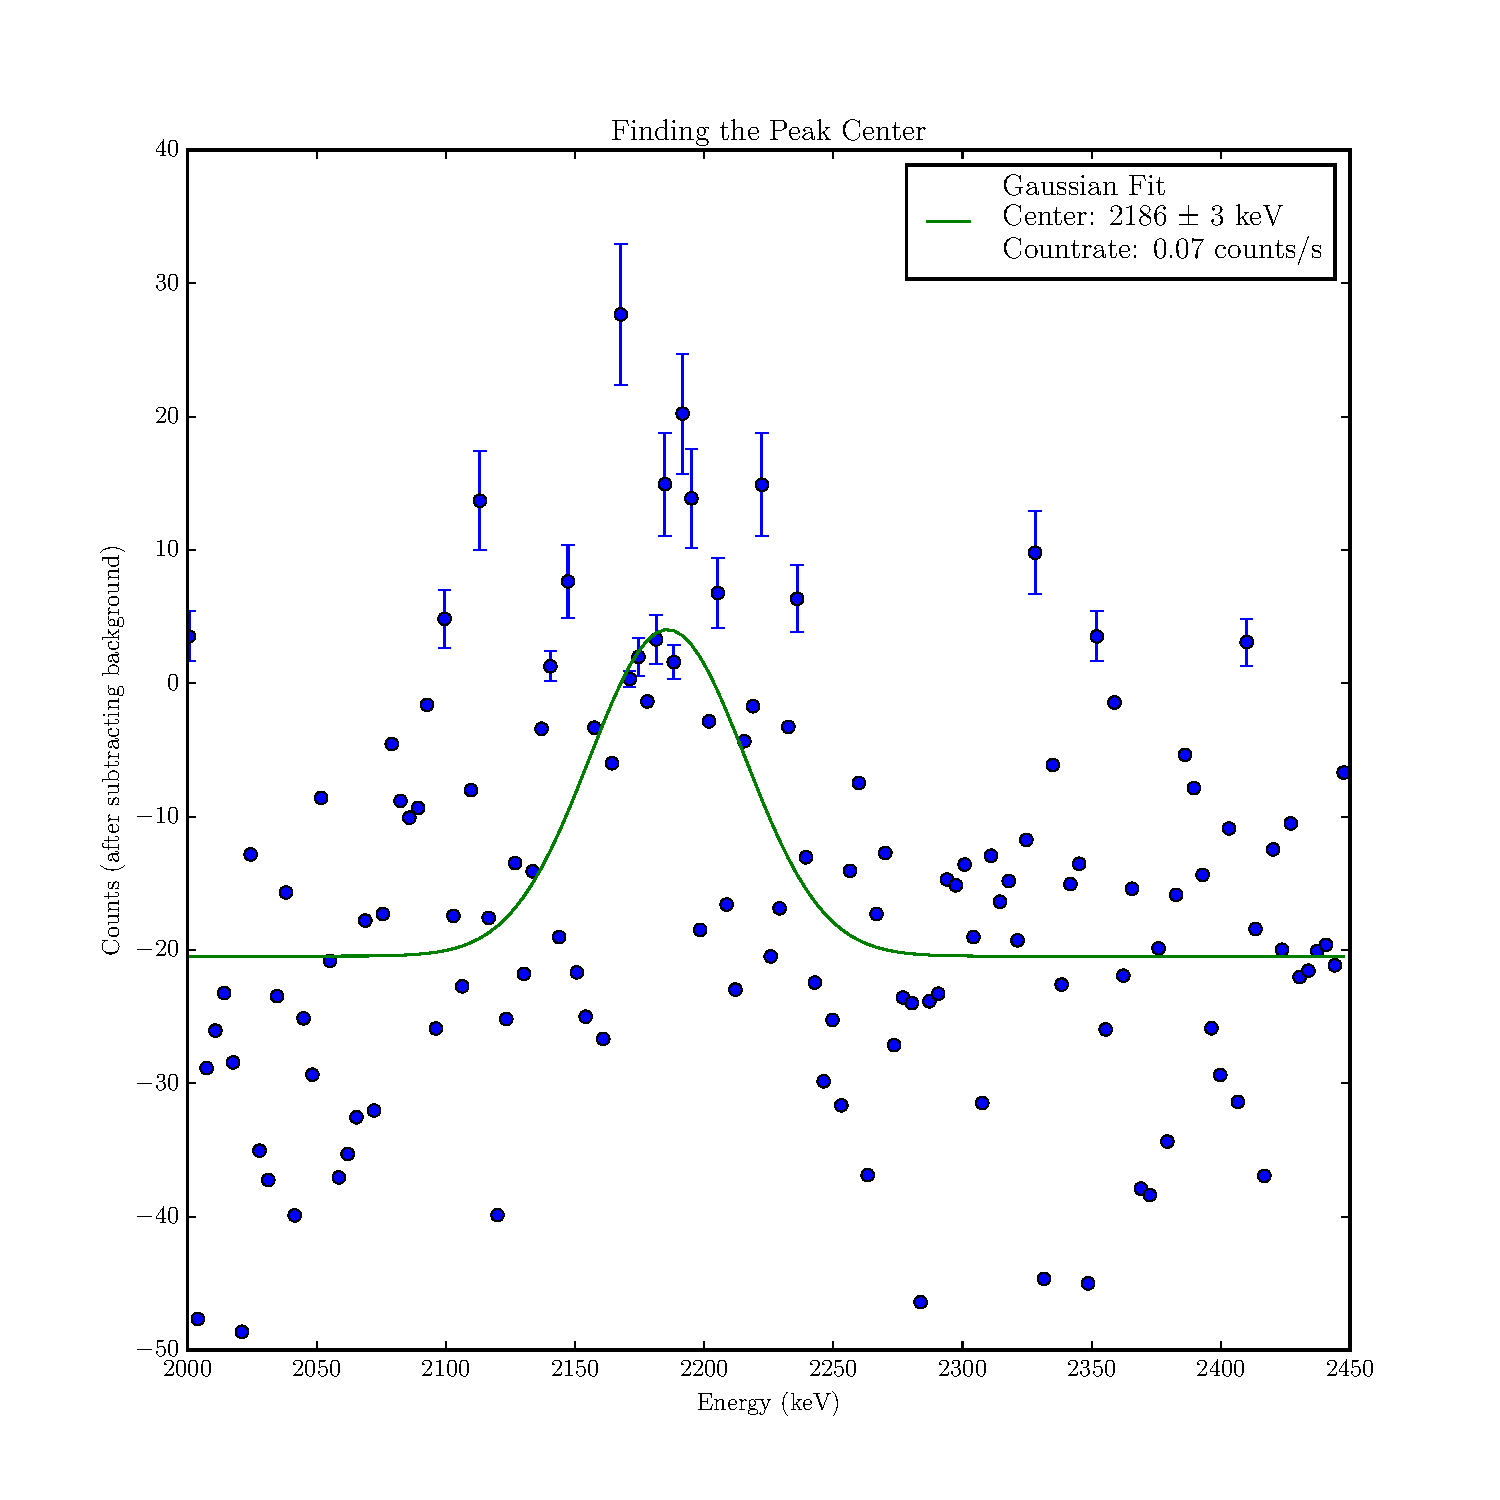
\includegraphics[scale=.4]{../plots/peak_center_shielded_carbon.pdf} \\
    \end{tabular}
    \caption{This peak is barely there.  We can see that the uncertainty on the fit is about 14\%, and even this is quite low for the true uncertainty.  We can see visually that if there is a peak there, it's miniscule and barely above the background level.  In fact, the spread from the lowest point to the highest point is roughly even about zero, there's almost no evidence of a peak at all.}
    \label{carbon}
  \end{figure}

  \begin{figure}[!htb]
    \begin{center}
      \begin{tabular}{c c}
        \begin{tabular}{c}
          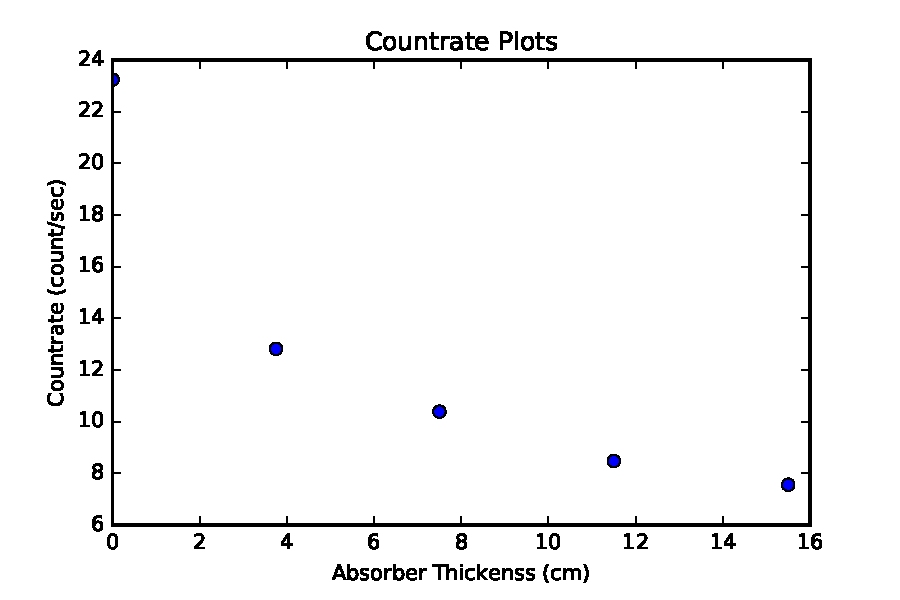
\includegraphics[width=.5\linewidth]{../plots/countrate_al.pdf} \\
          \small (a) Aluminum countrate; \redchi = 1.87
        \end{tabular}\label{rates:al} & \begin{tabular}{c}
          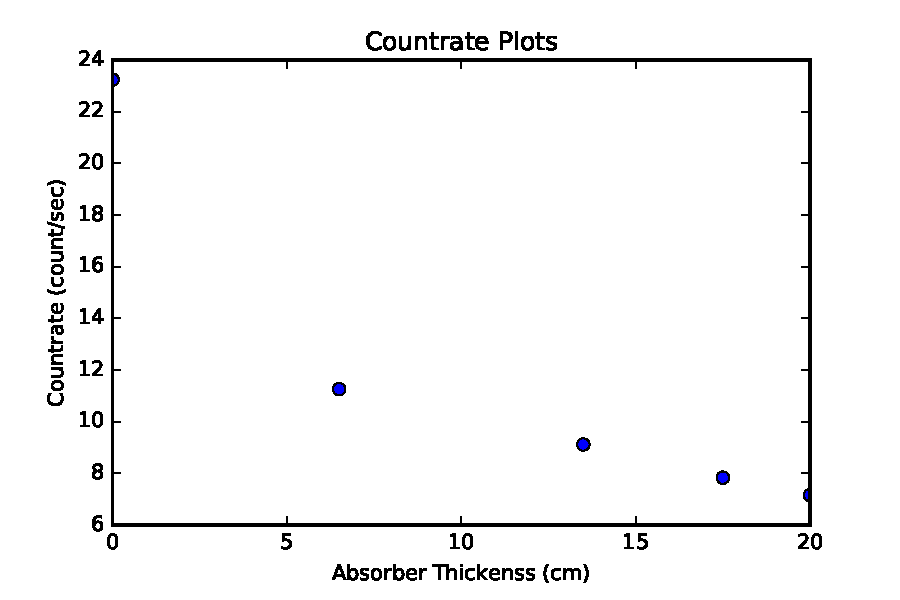
\includegraphics[width=.5\linewidth]{../plots/countrate_carbon.pdf} \\
          \small (b) Carbon countrate; \redchi = 2.21
        \end{tabular}\label{rates:carbon} \\
        \begin{tabular}{c}
          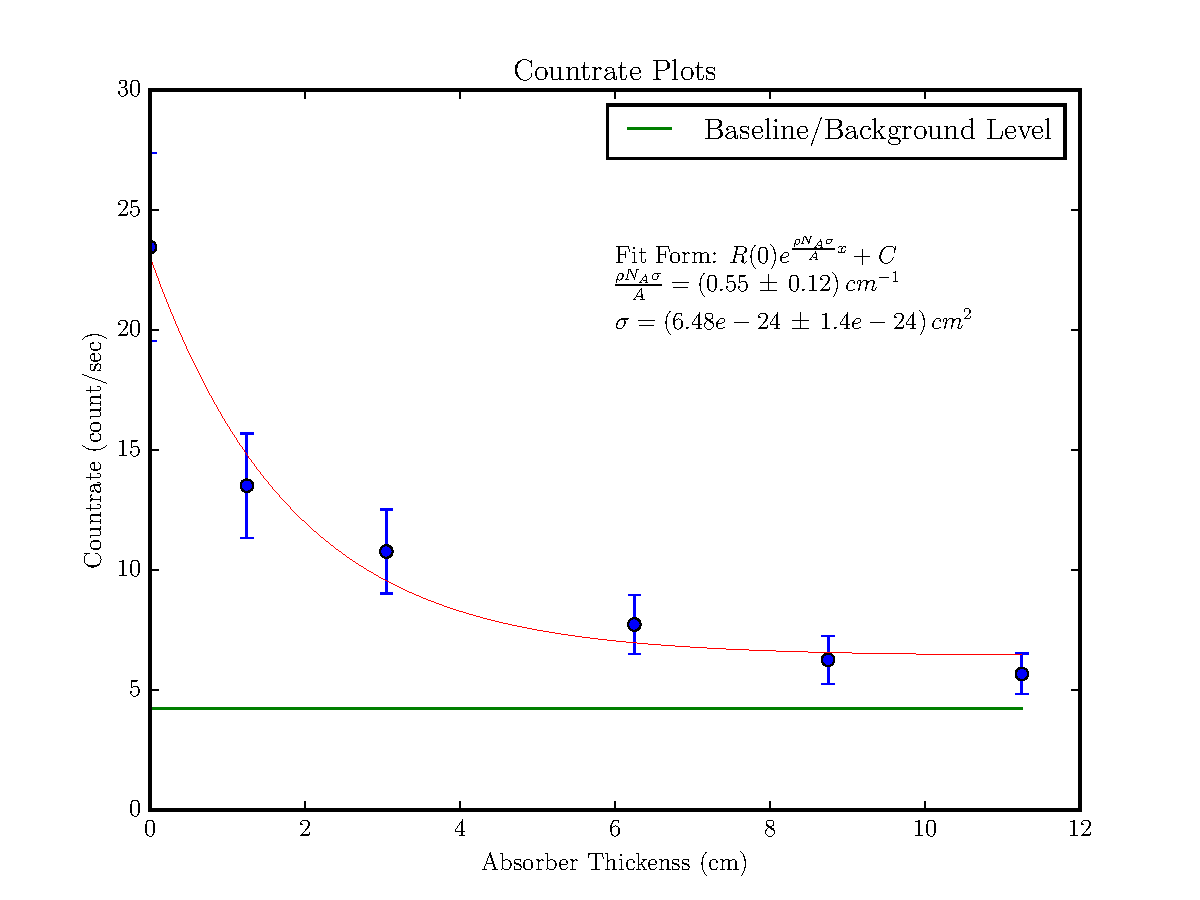
\includegraphics[width=.5\linewidth]{../plots/countrate_cu.pdf} \\
          \small (c) Copper countrate; \redchi = 5.69
        \end{tabular}\label{rates:cu} & \begin{tabular}{c}
          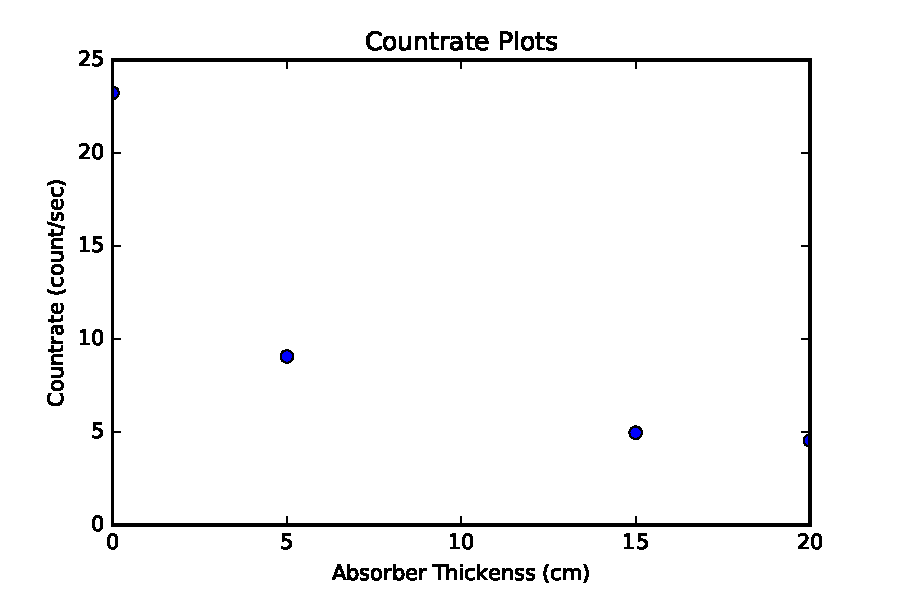
\includegraphics[width=.5\linewidth]{../plots/countrate_pb.pdf} \\
          \small (d) Lead countrate; \redchi = 0.93
        \end{tabular}\label{rates:pb}
      \end{tabular}
      \caption{As we can see, the fits are fairly good.  The \redchi values indicate good fits, and thus we are confident that the data does decay exponentially in the manner that we would expect.  The background level is shown in each plot simply to get an idea of what the background is.  For this level, we filled the absorber stand with as much lead as we could and took a spectrum.}
      \label{rates:rates}
    \end{center}
  \end{figure}

  \begin{figure}[!htb]
    \centering
    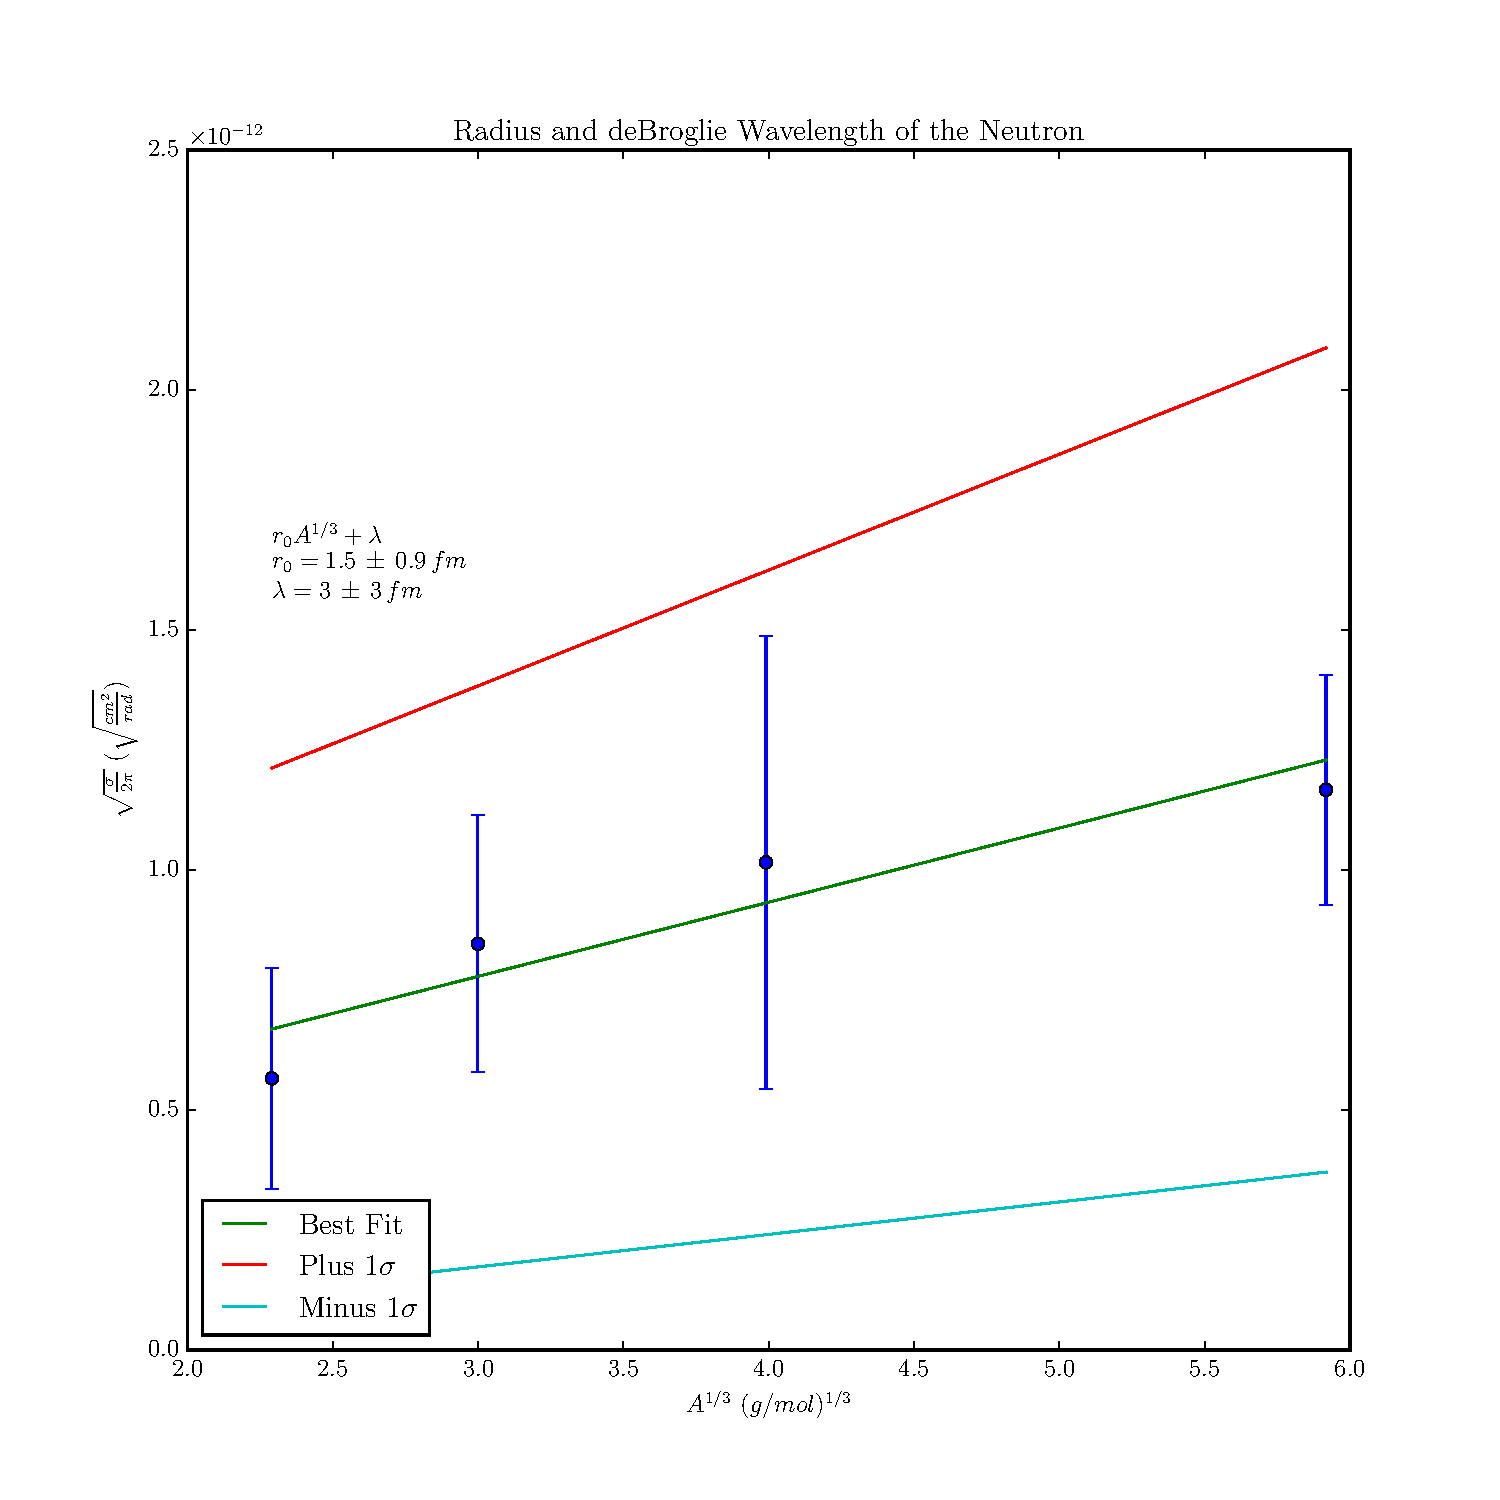
\includegraphics[scale=.7]{../plots/neutron_radius.pdf}
    \caption{The \redchi value for this fit is 1.02.  However, this is certainly due to the massive uncertainty in each value - which comes directly from uncertainty in the cross section.  We also show examples of lines with the best-fit slope and intercept plus and minus one standard deviation.}
    \label{radius}
  \end{figure}

\end{document}
